\documentclass[lettersize,journal]{IEEEtran}

\usepackage{amsmath,amsfonts,amssymb}
\usepackage{array}
\usepackage{stfloats}
\usepackage{url}
\usepackage{graphicx}
\usepackage{cite}
\newtheorem{theorem}{Theorem}
\newtheorem{proposition}{Proposition}
\newtheorem{corollary}{Corollary}
\newtheorem{remark}{Remark}
\hyphenation{op-tical net-works semi-conduc-tor IEEE-Xplore}
\def\BibTeX{{\rm B\kern-.05em{\sc i\kern-.025em b}\kern-.08em
    T\kern-.1667em\lower.7ex\hbox{E}\kern-.125emX}}

\urlstyle{same}
\begin{document}

\title{Multirobot Tracking of Separatrices and
Objective Eulerian Coherent Structures}

\author{Christopher Waight and Christopher A. Kitts,~\IEEEmembership{Senior Member,~IEEE}
\thanks{C. Waight is a PhD Candidate in the Robotic Systems Laboratory, Department of Mechanical Engineering, Santa Clara University, Santa Clara, CA 95053 USA (e-mail: cwaight@scu.edu)}
\thanks{C. A. Kitts is Professor and Director of the Robotic Systems Laboratory, Department of Mechanical Engineering, Santa Clara University, Santa Clara, CA 95053 USA (e-mail: ckitts@scu.edu)}
}
\markboth{IEEE Transactions on Robotics}%
{Waight and Kitts: Multirobot Tracking of Separatrices and Objective Eulerian Coherent Structures}

\maketitle

\begin{abstract}
Short-term transport in a geophysical flow is organized by
instantaneous coherent structures, curves of strongest local attraction
and repulsion, where drifting material collects within hours. Existing
robotic trackers either commit to a presumed structure in advance or
must integrate measurements over a time horizon before an estimate
exists. This paper presents a multirobot method for finding and
following these structures in real time, using only the instantaneous flow velocity
each robot measures at its own position. A cooperative estimator
recovers the local quadratic model of the field from one synchronous
measurement set, and six robots are proved to be the minimum team for
this recovery under the unconstrained quadratic model. The fit supplies two trackable surrogates. The first is the Jacobian
determinant, whose trenches trace the flow's separatrices. It is
Galilean invariant but not objective, shifting under a rotating observer, a liability for a team without a reliable global heading reference.
The second is the smaller rate-of-strain eigenvalue, whose trench is
objective, a material curve recovered identically in any observer frame.
An adaptive navigation controller rides each. A rotating-frame experiment
separates them. The strain tracker's inertial and rotating runs end
0.025 apart, while the determinant tracker's diverge by 1.219 as its
rotating-frame run leaves the structure. This objectivity has a
measurable cost in convergence rate and in noise tolerance at a single
decision point. Monte Carlo sweeps place the determinant
tracker's failure cliff at the estimator's own noise threshold,
$\sigma_{uv} \approx 0.01$, and the strain tracker's earlier, at
$\sigma_{uv} \approx 0.002$. At zero noise their tracking errors are
0.0016 and 0.0075. On Santa Barbara Channel radar currents, the
determinant tracker follows a coherent ridge for 28 hours to a consistent
landfall, and the strain tracker, started on that same ridge, rides the
same network structure from the objective strain term alone. Double-gyre
quantities are reported in the field's non-dimensional world units
throughout.
\end{abstract}

\begin{IEEEkeywords}
Multirobot Systems, Adaptive Navigation, Coherent Structures,
Okubo-Weiss, Rate of Strain, Objectivity, Cooperative
Estimation, Cluster Space Control
\end{IEEEkeywords}

\section{Introduction}
\label{sec:intro}

\IEEEPARstart{M}{ultirobot} systems (MRS) provide redundancy against
individual failures, widen the area a team can cover, and spread
sensing across space rather than concentrating it at a single
platform. These systems now operate across domains from warehousing
to search and rescue \cite{1}. Equipped with field sensors, such
teams form mobile sensor networks that turn spatial spread into
simultaneous measurements at separated points.

Survey-oriented navigation MRS use this ability to sweep a region
exhaustively and identify features only afterward. Adaptive navigation (AN) techniques instead use
measurements in real time to drive the network toward or along
features of interest, locating local features quickly and following
them as they evolve.

AN in scalar fields is well developed. Each robot contributes a single
scalar measurement to a navigation policy that reaches and follows
features such as extrema, contour lines, ridges, trenches, saddle
points, and fronts \cite{2,3,4,5}, with formations sized so that
differential measurements across the cluster recover the gradient and
curvature each policy consumes \cite{6,2}.

Some environments are better modeled by vector fields. These models
assign both a magnitude and a direction to each point. The critical
points of that vector field often mark the features a mission cares
about, for example, in ocean currents and other geophysical flows: a
sink can flag an area of high probability for search and rescue
\cite{7}, while a spewing vortex can point to a below-surface leak
\cite{8}.
In \cite{9}, a three-robot cluster estimated the location and type of
an isolated critical point from a linear fit of simultaneous local
velocity measurements, recovering the feature from instantaneous data
alone rather than from an accumulated survey.

Beyond isolated points, there is also utility in tracking extended
features such as fronts, dynamically meaningful lines along which
water masses converge. Coordinated multi-vehicle sampling of such
dynamic ocean features is itself an active area of marine robotics,
spanning drifter-referenced AUV surveys \cite{10}, front-tracking
ASV/AUV teams \cite{11}, and adaptive glider fleets \cite{12}.

Another line of great interest is the separatrix. In steady
two-dimensional flows it is the union of the stable and unstable
manifolds through the saddle points, partitioning the domain into
basins whose trajectories do not mix. Tracking it is relevant to
dispersion modeling, pollutant containment, and coastal sensor
deployment \cite{13,14,15}, and, like the related Okubo-Weiss field used
to classify oceanic mesoscale eddies \cite{16}, it can in principle be
inferred from instantaneous measurements alone.

A line of work on separatrix navigation has equipped robot teams to
track a coherent structure directly in the flow rather than
reconstruct it offline, by straddling a presumed manifold with a small
formation \cite{17,18,19,20} or by accumulating an onboard FTLE
estimate over a finite time horizon \cite{21}. Each approach either
commits to the structure's identity before tracking begins or pays an
integration latency before an estimate exists.

Two trackable surrogates of the flow's transport skeleton follow from
the local velocity gradient, the Jacobian determinant $D$ and the
smaller rate-of-strain eigenvalue $s_1$. $D$ is Galilean invariant but
not objective, while $s_1$ is objective, a distinction that matters
whenever a team cannot certify its own orientation against a trusted
external reference, as when a vehicle dead-reckons on a drifting compass
heading between GPS fixes or operates without GPS at all \cite{22,23}.
This paper makes four contributions. First, it presents a cooperative
second-order estimator that recovers the local quadratic model of a
two-component field from one synchronous sample, with six robots proved
minimal for the unconstrained quadratic model and with exact,
heading-isotropic noise gains. Second, it
develops the $D$ tracker, a hybrid controller built on a modified
Newton step that snaps onto a trench of $D$, slides along it, and
traverses the network of saddle crossings without committing to a
manifold identity in advance. Third, it develops the
$s_1$ tracker, an objective controller built from the strain
eigenframe whose design follows from the structural result that no
quadratic velocity fit can certify $s_1$-trench curvature.
Fourth, it validates both trackers under a fully specified
noise model, in a closed-loop rotating-frame objectivity experiment,
and on real Santa Barbara Channel radar currents.

The remainder of the paper is organized as follows. The rest of this
section reviews related work. Section~\ref{sec:detj_field} formulates
the problem. Section~\ref{sec:estimation} develops the six-robot
estimator and its accuracy under noise. Section~\ref{sec:controllers}
presents the two controllers and their stability properties.
Section~\ref{sec:methods}
describes the simulation program and test plan.
Section~\ref{sec:results} reports the results, including the ocean
experiments, and discusses their implications and limitations, and
Section~\ref{sec:conclusion} concludes.

\subsection{Related Work}
\label{sec:related_robots}

Haller and Yuan formalized the Lagrangian coherent structure (LCS) as
the generalization of stable and unstable manifolds to flows with
arbitrary time dependence \cite{13}. The standard computable definition,
a ridge of the finite-time Lyapunov exponent (FTLE) field, is given in
\cite{15} on the same double-gyre model used throughout this paper. The
objectivity and Lagrangian/Eulerian tradeoff that bears on any Eulerian
surrogate is developed in \cite{24,25,26}. Velocity-gradient
recovery from sparse trajectories \cite{27} and the strain-spin
decomposition itself \cite{28} remain active adjacent directions. The
instantaneous criteria remain the computable workhorses. Okubo and Weiss
partition a planar flow from the local velocity gradient alone
\cite{29,30}, generalized to three dimensions \cite{31}, refined for
oceanographic use \cite{32}, and used at scale in mesoscale eddy censuses
\cite{16}.

The nearest prior work tracks a coherent structure directly with a
robot formation. Michini et al. bracket a presumed stable or unstable
manifold with three robots using only local velocity measurements
\cite{17}. The strategy extends to $N$ robots \cite{18}, was validated
on micro surface vehicles in a flow tank \cite{19}, and related
flow-based control operates marine robots in gyre-like environments
\cite{20}. Unlike methods that sense only a scalar reduction of the
field \cite{33}, the team here fits the full local quadratic vector
field, so the surrogate's shape, not merely its sign, is available to
the controllers. The straddle family commits to the manifold's identity
before tracking begins, and neither controller nor proof addresses the
saddle point itself, exactly where that identity becomes ambiguous.
Kularatne and Hsieh instead compute the local FTLE field on board,
recovering the structure's type at the price of a nonzero integration
horizon \cite{21}. None of these strategies estimates the curvature of
the field itself, which is what fixes not just where a structure lies
but what kind it is and how many branches meet there.
Table~\ref{tab:assumptions} sets out the assumptions each of them
states, every cell sourced from the cited papers' own text. Two of the
rows are premises rather than details. \cite{17}'s straddling formation
control is stated for robots already on opposite sides of the boundary
and \cite{21} assumes the center robot starts on $B_u$, so neither
method's guarantee covers an off-structure start; and \cite{17,18,19,20}
and \cite{21} alike write the robot's velocity as the commanded term
plus the ambient flow, so their robots are advected.

\begin{table}[!t]
\centering
\caption{Stated assumptions, this paper against the nearest prior
robotic structure-tracking methods.}
\label{tab:assumptions}
\scriptsize
\setlength{\tabcolsep}{3pt}
\begin{tabular}{@{}l>{\raggedright\arraybackslash}p{0.19\linewidth}>{\raggedright\arraybackslash}p{0.19\linewidth}>{\raggedright\arraybackslash}p{0.19\linewidth}@{}}
\hline
& \textbf{This paper} & \textbf{\cite{17,18,19}} & \textbf{\cite{21}} \\
\hline
Init. & any six-robot config., on or off structure & straddling formation already on the manifold, opposite sides & center robot already on the boundary $B_u$ \\
Structure ID & not required in advance & assumed known (which boundary is straddled) & not required; located from the FTLE field itself \\
Sensing & one synchronous velocity sample per robot, no history & continuous velocity measurement per robot & a sensing grid advected over a finite window \\
Advection & robots not advected; field is sampled, not physically sat in & robots advected by the flow (their eq.~1a) & sensing grid particles advected by construction \\
Estimated & full local quadratic model: gradient and curvature of $D$ and $s_1$ & boundary crossing only, via a PIM triple & FTLE ridge location, via finite-time integration \\
Terminal behavior & traverses (both) or certifies a terminal core ($s_1$) & maintains the straddle; no terminal state & re-locates the ridge each window; no terminal state \\
\hline
\end{tabular}
\end{table}

The straddle family also reports its own limitation at the saddle.
Robots following \cite{17}'s strategy ``tend to veer away from the
tracked LCS as they approach a local saddle/hyperbolic point in the
flow,'' because ``the flow reverses direction on the other side of the
saddle point,'' in both their flow-tank and ocean trials.

On the estimation side, \"{O}gren, Fiorelli, and Leonard established
cooperative gradient climbing with a formation of mobile sensors
\cite{2}, and Bri\~{n}\'{o}n-Arranz, Renzaglia, and Schenato extended
the idea to the Hessian. Five robots on a ring plus one at the center
recover the gradient and Hessian of a scalar signal in closed form
\cite{6}. McDonald, Kitts, and Neumann developed the complementary
adaptive-navigation primitives that follow scalar-field ridges,
trenches, and saddle points from local differences alone
\cite{3,4,5}. Every one of these formations samples a single signal
channel. A coupled two-component field doubles the estimation problem
to twelve unknowns, which none of these formations addresses. Where
\cite{6} applies fixed symmetric weights valid
for the ideal ring geometry, the estimator here solves at the measured
positions and so stays exact even as the formation deforms. On the
control side, the step used here normalizes the Newton component by the
magnitude of the curvature in each eigendirection, a substitution that
also appears in the saddle-free method of Dauphin et al. \cite{34},
and takes the direction of the along-trench motion from the ambient
flow. The purpose differs. \cite{34} uses the substitution to escape
stationary points, while both trackers developed here are built to
find and hold them.

This paper and the critical-point and structure-tracking methods above
\cite{17,18,19,20,21,9} navigate a naturally occurring flow sensed in
situ, unlike the separate literature that builds an artificial vector
field as a synthetic guidance signal for single-robot path following
\cite{35} or obstacle avoidance \cite{36}.

\section{Problem Formulation}
\label{sec:detj_field}

\subsection{Vector Fields and Local Polynomial Models}

A planar vector field assigns a velocity vector $\mathbf{v}(\mathbf{p}) =
(u(\mathbf{p}), v(\mathbf{p}))$ to each position $\mathbf{p} = (x, y)$ in its
domain. The critical-point estimator of \cite{9} fits a \emph{planar}
(affine) model of each component to simultaneous measurements and solves
the linear system for the point where $\mathbf{v} = \mathbf{0}$. The
surrogates this paper tracks are built not from $\mathbf{v}$ but from its
spatial derivatives, and navigating them requires derivatives through
second order. A planar fit, whose second derivatives are identically zero,
cannot supply them.

The team therefore works from the second-order Taylor expansion of each
component about the cluster centroid $\mathbf{p}_c$. Coordinates
$\mathbf{p} = (x, y)$ are measured from the centroid throughout this
section, so that $\mathbf{p} = \mathbf{0}$ is the centroid itself.
\begin{align}
    u(\mathbf{p}) &= a_1 + a_2 x + a_3 y
        \nonumber \\
        &\quad + a_4 xy + \tfrac{1}{2} a_5 x^2 + \tfrac{1}{2} a_6 y^2
        + \mathcal{O}(\|\mathbf{p}\|^3),
        \label{eq:quad_model_u} \\
    v(\mathbf{p}) &= b_1 + b_2 x + b_3 y
        \nonumber \\
        &\quad + b_4 xy + \tfrac{1}{2} b_5 x^2 + \tfrac{1}{2} b_6 y^2
        + \mathcal{O}(\|\mathbf{p}\|^3).
        \label{eq:quad_model_v}
\end{align}
The twelve coefficients are constants. All position dependence in
(\ref{eq:quad_model_u})--(\ref{eq:quad_model_v}) is carried by $x$ and
$y$. Each coefficient is a derivative of the field at the centroid, and
the one-half factors are chosen so that the match is direct, giving
$a_1 = u(\mathbf{p}_c)$, $a_2 = \partial u/\partial x|_{\mathbf{p}_c}$,
$a_4 = \partial^2 u/\partial x \partial y|_{\mathbf{p}_c}$,
$a_5 = \partial^2 u/\partial x^2|_{\mathbf{p}_c}$, and likewise for
$b_1, \ldots, b_6$ with $v$ in place of $u$. Where a partial derivative
of the true field is meant rather than a fitted coefficient, this paper
writes it as a derivative, $u_x$, $u_{xy}$, and so on.

The team estimates these coefficients by fitting the quadratic model that
remains when the $\mathcal{O}(\|\mathbf{p}\|^3)$ remainder is discarded,
and marks the results with a hat. $\hat{a}_5$ is an estimate of $a_5$,
not the quantity itself. Two mechanisms separate them. Sensor
noise perturbs each measurement, and truncation bias arises because the
discarded cubic terms are not zero over a footprint of finite size, so the
fit absorbs part of them into the retained coefficients.

The first-order coefficients are the centroid values of the entries of the
field Jacobian
\begin{equation}
    \mathbf{J}(\mathbf{p}) =
    \begin{bmatrix}
        \partial u / \partial x & \partial u / \partial y \\
        \partial v / \partial x & \partial v / \partial y
    \end{bmatrix},
    \label{eq:jacobian}
\end{equation}
so that $\mathbf{J}_0 = \mathbf{J}(\mathbf{p}_c)$ has entries $a_2$,
$a_3$, $b_2$, $b_3$, and we write $D(\mathbf{p}) =
\det(\mathbf{J}(\mathbf{p}))$ throughout. 

\subsection{The Determinant Surrogate $D$}
\label{sec:separatrix}

The Okubo-Weiss parameter \cite{29,30}, built from the normal strain,
shear strain, and vorticity
($\omega = \partial v/\partial x - \partial u/\partial y$), satisfies
$Q = \tfrac{1}{4}(\nabla \cdot \mathbf{v})^2 - D$ by direct expansion.
For the incompressible flows considered here $Q = -D$ exactly, so we
work with $D$. The sign of $D$ fixes the local eigenstructure.
Incompressibility gives $\operatorname{tr}(\mathbf{J}) = 0$, so the
eigenvalues $\mu_J$ of $\mathbf{J}$ satisfy
\begin{equation}
    \mu_J = \pm\sqrt{-D} \ \ (D < 0), \qquad
    \mu_J = \pm i\sqrt{D} \ \ (D > 0).
    \label{eq:eig_detj}
\end{equation}
Where $D < 0$ the flow is locally hyperbolic (strain-dominated) and
nearby particles separate at the instantaneous exponential rate
$\sqrt{-D}$. Where $D > 0$ it is locally elliptic (rotation-dominated),
and the zero level set of $D$ is the Okubo-Weiss boundary between the
two regimes. The more negative $D$ is, the stronger the local
hyperbolicity, so trenches (valley lines) of $D$ inside strain regions
mark the loci of strongest instantaneous attraction and repulsion.

\subsection{The Strain-Eigenvalue Surrogate $s_1$}
\label{sec:strain_field}

The velocity gradient decomposes into symmetric and antisymmetric
parts, $\mathbf{J} = \mathbf{S} + \mathbf{W}$, with rate-of-strain
tensor $\mathbf{S} = (\mathbf{J} + \mathbf{J}^\top)/2$ and spin tensor
$\mathbf{W} = (\mathbf{J} - \mathbf{J}^\top)/2$, which carries the
vorticity. Consider a time-dependent change of observer
$\mathbf{p}' = \mathbf{Q}(t)\mathbf{p} + \mathbf{b}(t)$, with rotating
frame $\mathbf{Q}(t)$. For the special case
$\mathbf{p}' = \mathbf{Q}(t)\mathbf{p}$, the convention used in the
rotating-frame experiment of Section~\ref{sec:test_plan}, write
$\dot{\mathbf{Q}}\mathbf{Q}^\top = \Omega\left[\begin{smallmatrix} 0 &
-1 \\ 1 & 0 \end{smallmatrix}\right]$, so $\Omega$ is the frame's own
angular rate. The frame's rotation enters the velocity gradient only
through this antisymmetric term, so it lands entirely in the spin
part, $\omega' = \omega + 2\Omega$, while the strain part transforms
cleanly, $\mathbf{S}' = \mathbf{Q}\mathbf{S}\mathbf{Q}^\top$. The
eigenvalues $s_1 \leq s_2$ of $\mathbf{S}$ are therefore
frame-invariant, its eigenvectors $\mathbf{e}_1, \mathbf{e}_2$
co-rotate with the frame, and quantities built from them are
objective. Material behavior, which cannot depend on the observer, can
be predicted from them in any frame \cite{24,25}.

The two surrogates of this paper are the two halves of this splitting.
For any symmetric $\mathbf{S}$ and antisymmetric $\mathbf{W}$ the cross
term vanishes, $\operatorname{tr}(\mathbf{S}\mathbf{W}) = 0$, so the
determinant splits exactly.
\begin{equation}
    D \;=\; \det\mathbf{S} + \det\mathbf{W}
      \;=\; s_1 s_2 + \frac{\omega^2}{4}
      \;=\; \frac{\omega^2}{4} - s_1^2,
    \label{eq:splitting}
\end{equation}
the last equality by incompressibility ($s_2 = -s_1$). Three
consequences of (\ref{eq:splitting}) organize everything that follows.
First, the Okubo-Weiss partition is the competition between the two
terms, rotation-dominated where the spin term wins ($D > 0$),
strain-dominated where the strain term wins ($D < 0$). Second,
substituting $\omega' = \omega + 2\Omega$ gives
\begin{equation}
    D' = D + \Omega\,\omega + \Omega^2,
    \label{eq:D_not_objective}
\end{equation}
so two observers rotating relative to one another disagree about where
the $D$ structures are. The frame artifact lives entirely in the spin
term, and its size relative to the flow's own rotation is set by the
Rossby number, taken here as the ratio of the frame's contribution to the
vorticity scale of the field,
\begin{equation}
    \mathrm{Ro} = \frac{2\Omega}{\lvert\omega\rvert_{\max}} .
    \label{eq:rossby}
\end{equation}
Every quantity derived from $D$ therefore carries a relative
frame-dependence of order $\mathrm{Ro}$, and every quantity derived from
$s_1$ carries none. For the rotating-frame experiment of
Section~\ref{sec:test_plan}, $2\Omega = 0.4$ against the double gyre's
peak vorticity $2\pi^2 A \approx 1.97$, so $\mathrm{Ro} \approx 0.20$.
Third, where the vorticity vanishes the identity collapses to
$s_1 = -\sqrt{-D}$. The two surrogates coincide on vorticity-free
lines and part ways everywhere else.

The smaller eigenvalue $s_1$ is the local instantaneous contraction
rate. Where $s_1 < 0$, material filaments are compressed along
$\mathbf{e}_1$ and stretched along $\mathbf{e}_2$ at rate $s_2 = -s_1$.
An attracting objective Eulerian coherent structure (OECS) is a trench
of the signed scalar field $s_1$ ridden along the stretching eigenvector
$\mathbf{e}_2$, a curve on which $s_1 < 0$ is locally most negative in
the transverse direction, so neighboring material is drawn onto it
\cite{25}. This is the objective counterpart of the $D$ trench.

One caution accompanies the eigenstructure. $\mathbf{e}_1, \mathbf{e}_2$ are direction fields
with no globally consistent sign, undefined at isotropic points of
$\mathbf{S}$ ($s_1 = s_2$), so the controller must orient its tangent by
continuity rather than by any pointwise rule.

\subsection{The Double-Gyre Example}
\label{sec:dg_example}

The double-gyre flow used throughout is the steady ($\varepsilon = 0$)
member of the Shadden family \cite{15}, shifted from the canonical domain
$[0,2] \times [0,1]$ to $[-1,1] \times [-0.5, 0.5]$ by
$x_f = x + 1$, $y_f = y + 0.5$, where $(x_f, y_f)$ are field-frame and
$(x, y)$ world-frame coordinates. Both are non-dimensional throughout the
double-gyre experiments, so distances and gaps reported in world-frame
units (Section~\ref{sec:results}) carry no
further unit conversion unless stated. The field is
\begin{equation}
    u = -\pi A \sin(\pi x_f) \cos(\pi y_f), \quad
    v = \pi A \cos(\pi x_f) \sin(\pi y_f),
    \label{eq:dg_u}
\end{equation}
with $A = 0.1$. The flow is incompressible, the separatrix is the line
$x = 0$, the saddle points are $\mathbf{p}^*_1 = (0, -0.5)$ and
$\mathbf{p}^*_2 = (0, 0.5)$, and the gyre centers are $(\pm 0.5, 0)$.

All quantities of interest have closed forms. The Jacobian entries are
$u_x = -\pi^2 A \cos\pi x_f \cos\pi y_f = -v_y$ and
$u_y = \pi^2 A \sin\pi x_f \sin\pi y_f = -v_x$, so the flow is divergence
free, and direct differentiation of (\ref{eq:dg_u}) with the double-angle
identities gives
\begin{equation}
    D(\mathbf{p}) = -\frac{\pi^4 A^2}{2}
    \bigl(\cos 2\pi x_f + \cos 2\pi y_f\bigr),
    \label{eq:det_analytic_main}
\end{equation}
\begin{equation}
    \begin{aligned}
    \nabla D &= \pi^5 A^2
    \begin{bmatrix} \sin 2\pi x_f \\ \sin 2\pi y_f \end{bmatrix},
    \\
    \mathbf{H}_D &= 2\pi^6 A^2
    \begin{bmatrix} \cos 2\pi x_f & 0 \\ 0 & \cos 2\pi y_f \end{bmatrix}.
    \end{aligned}
    \label{eq:gradhess_analytic_main}
\end{equation}
with vorticity $\omega = -2\pi^2 A \sin\pi x_f \sin\pi y_f$. Three facts
follow directly. First, the Okubo-Weiss boundary is the diamond
$x_f \pm y_f \in \tfrac{1}{2} + \mathbb{Z}$ inscribed around each gyre
center, $D > 0$ inside.

Second, the separatrix is a trench of $D$. Cross-track curvature
$2\pi^6 A^2 > 0$ on $x = 0$ (Fig.~\ref{fig:trench_cross}), deepest at
the two saddles, rising to a crest ($D = 0$, vorticity also zero, so
$\sqrt{-D}$ by (\ref{eq:splitting}) is the attraction rate toward it)
at the origin, where a descend-only controller stalls. Periodicity
turns the trenches of $D$ into a grid whose right-angle crossings
are the saddle points, so a tracker continuing past a saddle is still
on a trench (Sections~\ref{sec:stability} and \ref{sec:results}).

Third, the strain field shares the grid but signs its segments. The
shear strain vanishes identically, so $\mathbf{S} =
\mathrm{diag}(u_x, -u_x)$ everywhere, eigenvectors fixed on the
coordinate axes away from the degeneracy lines
$\cos\pi x_f \cos\pi y_f = 0$, giving
\begin{equation}
    s_1 = -\pi^2 A\,\lvert\cos \pi x_f \cos \pi y_f\rvert,
    \label{eq:s1_analytic_main}
\end{equation}
with the trench minima $s_1 = -\pi^2 A$ at the six flow saddles, the
terminal cores a traverse settles at, the two interior saddles
$\mathbf{p}^*_1$, $\mathbf{p}^*_2$ and, by the periodicity of
(\ref{eq:det_analytic_main}), the four further crossings the domain
walls carry at $x = \pm 1$, $y = \pm 0.5$.
Equation~(\ref{eq:s1_analytic_main}) shows $s_1$ is a transverse trench
of the separatrix on \emph{both} halves, with no sign change and no
ridge to cross. What alternates by segment is the \emph{material}
identity of its tangent, the stretching eigenvector $\mathbf{e}_2$ above
and the compression eigenvector $\mathbf{e}_1$ below, swapping at the
origin, the isotropic point of $\mathbf{S}$ where the $D$ crest sits
and $\mathbf{e}_1, \mathbf{e}_2$ are simultaneously undefined. An
objective tracker that keys its transverse channel to the trench of
$s_1$ rather than to a named eigenvector needs no ridge detector and no
special handling at the isotropic point. The same law holds the same
scalar trench on both halves, and the crossing itself is a genuine
two-dimensional minimum of $s_1$.

\begin{figure}[!t]
    \centering
    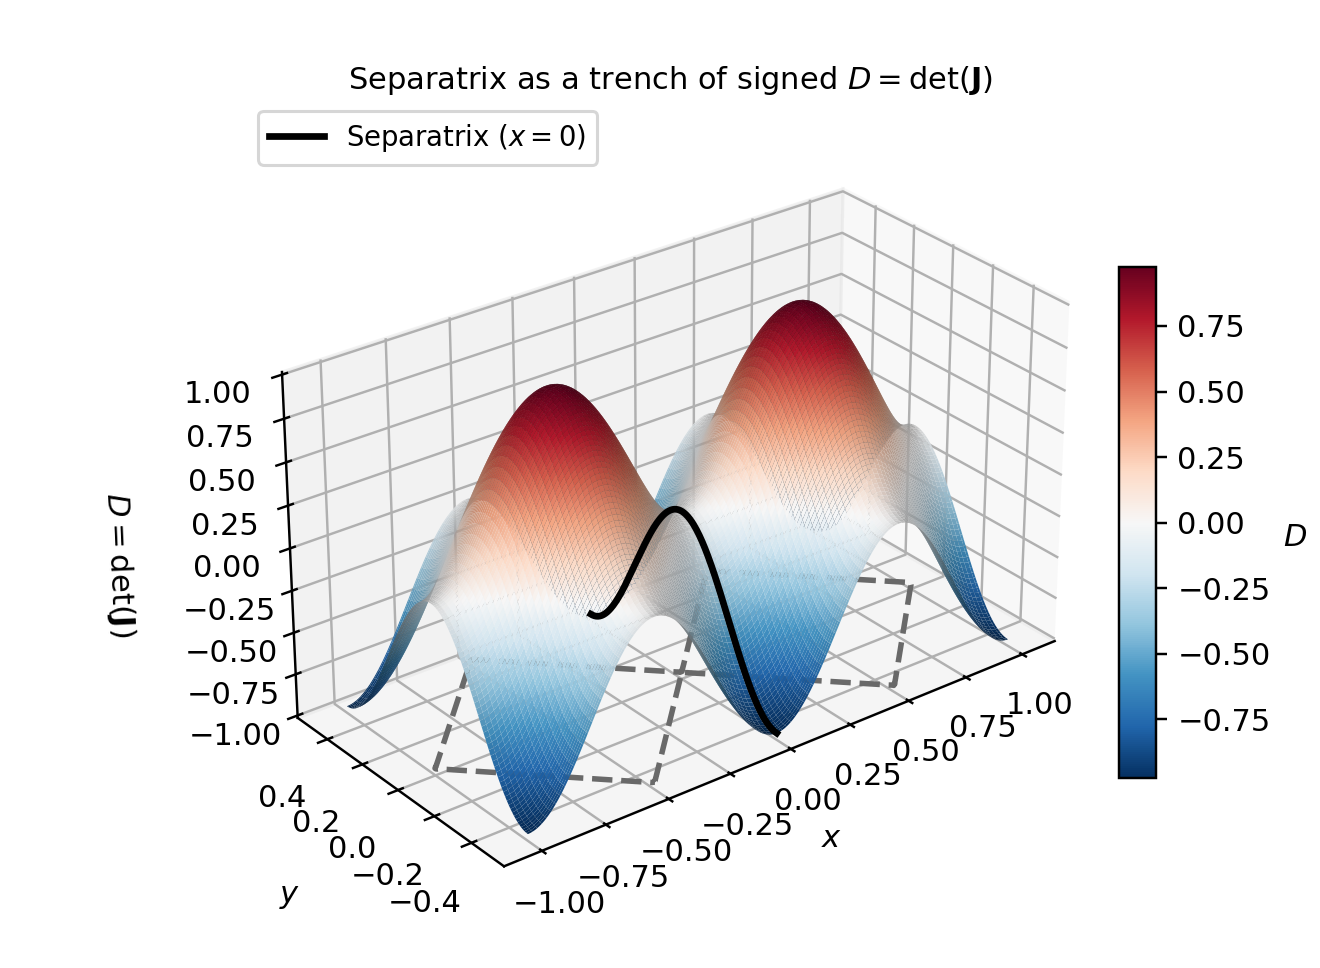
\includegraphics[width=0.36\textwidth]{figures/detJ_trench_cross_section.png}
    \caption{Signed $D$ as an elevation surface over the double gyre.
    The gyre cores rise as ridges ($D > 0$). The separatrix at $x = 0$
    (bold) is a trench of $D$, deepest at the saddles and rising to
    $D = 0$ at the origin.}
    \label{fig:trench_cross}
\end{figure}

\subsection{Problem Statement}
\label{sec:problem_statement}

Consider six robots at positions $\mathbf{p}_i$, the minimum team
Proposition~\ref{prop:minimality} establishes for this recovery, each
measuring the local flow $(u_i, v_i) = \mathbf{v}(\mathbf{p}_i)$ at the
common sampling instant, with no map, forecast, or prior field model and no
trajectory integration. The measured flow is a sampled datum, not a
current that advects the platform. Robot motion is commanded by the
control law, not advected by the sampled flow. Using
only the current synchronous samples at
each control cycle, the team must generate a centroid velocity command
$\dot{\mathbf{p}}_c$ that solves one of two problems, one per term of
(\ref{eq:splitting}).

\emph{Problem 1 (separatrix network traversal).} Drive the cluster
centroid onto the trench of $D$ and travel it, in the direction of the
ambient flow, through the saddle points where trench segments cross.

\emph{Problem 2 (objective network traversal).} Drive the centroid onto
the trench of $s_1$ and travel it, through the isotropic point where the
attracting and repelling segments meet, and certify a terminal
attracting core where one is reachable, using only objective quantities
throughout.


\section{Cooperative Second-Order Estimation}
\label{sec:estimation}

\subsection{Quadratic Fit from Six Simultaneous Measurements}

With robot positions $\mathbf{p}_i = (x_i, y_i)$ again measured from the
centroid, define the quadratic basis vector
\begin{equation}
    \boldsymbol{\phi}(\mathbf{p}) =
    \bigl[\,1, \; x, \; y, \; xy, \;
    \tfrac{1}{2}x^2, \; \tfrac{1}{2}y^2\,\bigr]^\top,
    \label{eq:basis}
\end{equation}
whose entries are the terms of
(\ref{eq:quad_model_u})--(\ref{eq:quad_model_v}) in the same order, so
the recovered coefficients estimate the Taylor derivatives directly with
no rescaling. Stacking the six robots' basis vectors row-wise gives
the $6 \times 6$ formation matrix $\boldsymbol{\Phi}$, and the coefficient
estimates $\hat{\boldsymbol{\theta}}_u = [\hat{a}_1, \ldots,
\hat{a}_6]^\top$ and $\hat{\boldsymbol{\theta}}_v = [\hat{b}_1, \ldots,
\hat{b}_6]^\top$ solve
\begin{equation}
    \boldsymbol{\Phi}\,\hat{\boldsymbol{\theta}}_u = \mathbf{m}_u, \qquad
    \boldsymbol{\Phi}\,\hat{\boldsymbol{\theta}}_v = \mathbf{m}_v,
    \label{eq:solve}
\end{equation}
where $\mathbf{m}_u = [u_1, \ldots, u_6]^\top$ and
$\mathbf{m}_v = [v_1, \ldots, v_6]^\top$ collect the measurements, $u_i$
and $v_i$ being the field components sampled by robot $i$. One matrix
factorization serves both components. If the field is exactly quadratic
over the formation footprint, the $\mathcal{O}(\|\mathbf{p}\|^3)$
remainder vanishes identically, and noise-free measurements give
$\hat{\boldsymbol{\theta}}_u = \boldsymbol{\theta}_u$ and
$\hat{\boldsymbol{\theta}}_v = \boldsymbol{\theta}_v$ for any nonsingular
$\boldsymbol{\Phi}$. Neither condition holds exactly in practice.

\begin{proposition}[Minimality]
\label{prop:minimality}
A synchronous sample from fewer than six robots leaves the
unconstrained quadratic model unidentifiable.
\end{proposition}

\begin{IEEEproof}
Each robot contributes one equation per component to (\ref{eq:solve}),
and each system has six unknowns, so fewer than six robots leave the
solution set a positive-dimensional affine subspace.
\end{IEEEproof}

Any method returning a single answer from five robots is therefore
supplying a structural prior rather than reading one from the data. Such
a prior is available. Imposing exact incompressibility ties $a_2 + b_3 =
0$ together with its two first derivatives, removing three coefficients,
so five robots then supply ten equations for nine unknowns. The
estimator fits the unconstrained model deliberately. The refusal to
presuppose that motivates the rest of the method is extended here to
the constitutive assumption about the field. Neither pre-straddling an
assumed manifold nor accumulating data points is required
(Section~\ref{sec:related_robots}), and the sixth robot buys the same
independence from a constitutive assumption about the field, exactness
over every planar quadratic field rather than only over an incompressible
subclass.

Six robots suffice exactly when $\boldsymbol{\Phi}$ is nonsingular, and
the singular formations admit a clean geometric description.

\begin{proposition}[Conic criterion]
\label{prop:conic}
$\boldsymbol{\Phi}$ is singular if and only if the six sampling points
lie on a common conic, including degenerate conics such as line pairs.
\end{proposition}

\begin{IEEEproof}
$\boldsymbol{\Phi}$ is singular exactly when
$\boldsymbol{\Phi}\mathbf{c} = \mathbf{0}$ for some nonzero
$\mathbf{c} \in \mathbb{R}^6$. Row $i$ of $\boldsymbol{\Phi}$ is
$\boldsymbol{\phi}(\mathbf{p}_i)^\top$, so this holds if and only if
$\boldsymbol{\phi}(\mathbf{p}_i)^\top \mathbf{c} = 0$ for every $i$,
that is, if and only if all six points lie on the zero set of the nonzero
quadratic polynomial $\boldsymbol{\phi}(\cdot)^\top \mathbf{c}$.
\end{IEEEproof}

The criterion carries a practical warning. Any six robots on one circle,
a regular hexagon for example, are singular regardless of size or
orientation. Moving one robot to the center removes the degeneracy
entirely.

\begin{corollary}[Pentagon-plus-center]
\label{cor:pentagon}
The pentagon-plus-center formation, five robots on a ring of radius
$\rho$ at $72^\circ$ spacing and one at the center, is nonsingular.
\end{corollary}

\begin{IEEEproof}
A conic vanishing at five points of a circle must be a multiple of that
circle, and a circle does not pass through its own center, so the six
points lie on no common conic.
\end{IEEEproof}

This is the configuration \cite{6} derived for scalar Hessian
estimation, whose
fixed symmetric weights are exact only for the ideal ring geometry and
bias the recovered Hessian under formation deformation. Solving
(\ref{eq:solve}) at the measured positions instead costs one
$6 \times 6$ factorization per cycle, reused for
both components, and stays exact under any deformation short of the
conic degeneracy, with formation error entering only through the
conditioning of $\boldsymbol{\Phi}$ (Section~\ref{sec:limitations}).

\subsection{Closed-Form Recovery of $D$, $\nabla D$, and $\mathbf{H}_D$}

The estimated Jacobian at the centroid is assembled from the linear
coefficients,
\begin{equation}
    \hat{\mathbf{J}}_0 =
    \begin{bmatrix}
        \hat{a}_2 & \hat{a}_3 \\ \hat{b}_2 & \hat{b}_3
    \end{bmatrix},
    \qquad
    \hat{D}_0 = \hat{a}_2 \hat{b}_3 - \hat{a}_3 \hat{b}_2.
    \label{eq:J_hat}
\end{equation}
Away from the centroid the fitted model makes every Jacobian entry affine
in position,
\begin{equation}
    \hat{\mathbf{J}}(\mathbf{p}) = \hat{\mathbf{J}}_0 +
    \begin{bmatrix}
        \hat{a}_5 x + \hat{a}_4 y &
        \hat{a}_4 x + \hat{a}_6 y \\
        \hat{b}_5 x + \hat{b}_4 y &
        \hat{b}_4 x + \hat{b}_6 y
    \end{bmatrix},
    \label{eq:jac_affine}
\end{equation}
so $\hat{D}(\mathbf{p}) = \det(\hat{\mathbf{J}}(\mathbf{p}))$ is an exactly
quadratic polynomial in position over the footprint. Differentiating
it and evaluating at the centroid $\mathbf{p} = \mathbf{0}$ gives the
gradient and Hessian there as polynomials in the fitted coefficients.
\begin{equation}
    \hat{\mathbf{g}}_0 =
    \begin{bmatrix}
        \hat{a}_5 \hat{b}_3 + \hat{a}_2 \hat{b}_4
            - \hat{a}_4 \hat{b}_2 - \hat{a}_3 \hat{b}_5 \\
        \hat{a}_4 \hat{b}_3 + \hat{a}_2 \hat{b}_6
            - \hat{a}_6 \hat{b}_2 - \hat{a}_3 \hat{b}_4
    \end{bmatrix},
    \label{eq:grad_det}
\end{equation}
\begin{equation}
    \hat{\mathbf{H}}_{D,0} =
    \begin{bmatrix}
        2(\hat{a}_5 \hat{b}_4 - \hat{a}_4 \hat{b}_5) &
        \hat{a}_5 \hat{b}_6 - \hat{a}_6 \hat{b}_5 \\
        \hat{a}_5 \hat{b}_6 - \hat{a}_6 \hat{b}_5 &
        2(\hat{a}_4 \hat{b}_6 - \hat{a}_6 \hat{b}_4)
    \end{bmatrix}.
    \label{eq:hess_det}
\end{equation}
Because $\hat{D}$ is quadratic, $\hat{\mathbf{H}}_{D,0}$ is independent of
position, the model reports the same curvature everywhere in the
footprint, and unlike the gradient it does not sharpen as the cluster
contracts onto the target. With the estimated flow at the centroid,
$\hat{\mathbf{v}}_0 = (\hat{a}_1, \hat{b}_1)$,
(\ref{eq:J_hat})--(\ref{eq:hess_det}) supply every quantity the $D$
tracker consumes.



\subsection{Closed-Form Recovery of $s_1$ and the Strain Eigenframe}
\label{sec:s1_estimation}

The same fit supplies the objective strain quantities. Write $\mu$,
$s_n$, and $s_s$ for the
mean, deviatoric normal, and shear strain, which the fitted first-order
coefficients give as
\begin{equation}
    \mu = \frac{\hat{a}_2 + \hat{b}_3}{2}, \quad
    s_n = \frac{\hat{a}_2 - \hat{b}_3}{2}, \quad
    s_s = \frac{\hat{a}_3 + \hat{b}_2}{2},
    \label{eq:strain_parts}
\end{equation}
with $\mu = 0$ for incompressible flow. The strain eigenvalues are
$s_{1,2} = \mu \mp r$ with $r = \sqrt{s_n^2 + s_s^2}$, and the
eigenframe $(\mathbf{e}_1, \mathbf{e}_2)$ is that of the symmetric
matrix $\hat{\mathbf{S}}$ assembled from the same coefficients. Every
quantity in this subsection is read from the fit. Hats are written where
an estimate is contrasted with its clean value, as in
Section~\ref{sec:sensitivity}, and suppressed on $\mu$, $s_n$, $s_s$,
$r$, and the eigenvectors elsewhere. Under
the quadratic model, $\mu$, $s_n$, and $s_s$ are affine functions of
position, so the gradient of $\hat{s}_1$ is exact for the fitted field.
\begin{equation}
    \nabla \hat{s}_1 = \nabla\mu
    - \frac{s_n\,\nabla s_n + s_s\,\nabla s_s}{r},
    \label{eq:grad_s1}
\end{equation}
with $\nabla\mu$, $\nabla s_n$, $\nabla s_s$ read directly off the
second-order coefficients (for example $\nabla s_n = \tfrac{1}{2}
(\hat{a}_5 - \hat{b}_4,\; \hat{a}_4 - \hat{b}_6)^\top$).



\begin{remark}[No usable Hessian of $s_1$ exists under a quadratic fit]
\label{rem:s1hess}
A Newton step on $(\nabla \hat{s}_1,
\hat{\mathbf{H}}_{s_1})$ is impossible in principle, not merely
inaccurate. Under the quadratic model the map $\mathbf{p} \mapsto (s_n,
s_s)$ is affine, so $\hat{s}_1 = \mu - \|(s_n, s_s)\|$ is concave and its
Hessian is negative semidefinite \emph{for every field and every
formation}. The positive transverse curvature of an $s_1$ trench lives
in third derivatives of the velocity field, outside the span of any
quadratic fit. (On the double gyre, where $s_s \equiv 0$, the fitted
$\hat{\mathbf{H}}_{s_1}$ is numerically zero.) The gradient
(\ref{eq:grad_s1}) is unaffected. Its transverse component recovers the
trench-restoring signal with the correct sign.
\end{remark}

\subsection{Estimator Sensitivity}
\label{sec:sensitivity}

Two noise channels perturb the samples. The first is measurement noise,
additive and Gaussian on the field components each robot reads:
\begin{equation}
    u_i^m = u(\mathbf{p}_i) + \eta_i^u, \quad
    v_i^m = v(\mathbf{p}_i) + \eta_i^v,
    \quad \eta \sim \mathcal{N}(0, \sigma_{uv}^2),
    \label{eq:meas_noise}
\end{equation}
where $\eta_i^u$ and $\eta_i^v$ are independent across robots,
components, and control cycles, following the sensor model of \cite{17}.
The second is position noise, which perturbs where each robot samples
rather than what it reads:
\begin{equation}
    (u_i^m, v_i^m) = \mathbf{v}(\mathbf{p}_i + \boldsymbol{\xi}_i), \quad
    \boldsymbol{\xi}_i \sim \mathcal{N}(\mathbf{0}, \sigma_p^2 \mathbf{I}),
    \label{eq:pos_noise}
\end{equation}
while the fit (\ref{eq:solve}) uses the nominal positions
$\mathbf{p}_i$. To first order, a displaced robot commits a reading
error $\mathbf{J}\boldsymbol{\xi}_i$, so at that order the two channels
combine into a single effective level:
\begin{equation}
    \sigma_{\mathrm{eff}}^2 = \sigma_{uv}^2
        + \tfrac{1}{2}\lVert\mathbf{J}\rVert_F^2\,\sigma_p^2 .
    \label{eq:sigma_eff}
\end{equation}
Noise reaches the tracked quantities through three maps, and each map
propagates it differently: the fit is linear, the determinant is
bilinear, and the strain eigenvalue is neither.

The fit is linear in the measurements. Solving (\ref{eq:solve}) gives
$\hat{\boldsymbol{\theta}} = \boldsymbol{\theta}^0 +
\boldsymbol{\Phi}^{-1}\boldsymbol{\eta}$ exactly, where
$\boldsymbol{\theta}^0$ denotes the coefficients the same fit returns on
clean measurements, so the noise gains are the row norms of
$\boldsymbol{\Phi}^{-1}$. For the pentagon-plus-center formation, a
coefficient of derivative order $q$ has standard deviation
\begin{equation}
    \sigma_{\theta_q} = \gamma_q\,
    \frac{\sigma_{\mathrm{eff}}}{\rho^{\,q}},
    \qquad
    \gamma_0 = 1, \;\;
    \gamma_1 = \tfrac{2}{\sqrt{10}}, \;\;
    \gamma_2 = \tfrac{8}{\sqrt{10}},
    \label{eq:gain_ladder}
\end{equation}
where $\gamma_2 = 4/\sqrt{10}$ for the mixed coefficient. These
constants follow from the symmetry of the ring: each entry of
$\boldsymbol{\Phi}^\top\boldsymbol{\Phi}$ is a ring sum of a monomial of
degree at most four, the odd sums vanish, and the even sums are
constants independent of ring phase. As a result the linear block
separates from the rest, its two rows are orthogonal with equal norm,
and the gradient covariance is
$\tfrac{4}{10}\sigma_{\mathrm{eff}}^2\rho^{-2}\mathbf{I}$, isotropic at
every heading. Only the constants $\gamma_q$ are specific to this
formation; the exponent is not, because recovering a derivative of order
$q$ costs $q$ difference quotients while only the signal scales with
$\rho$.

The determinant is bilinear in the fitted coefficients, which fixes the
behavior of every quantity the $D$ tracker consumes.

\begin{proposition}[Noise adds no bias to the $D$ family]
\label{prop:unbiased}
Under (\ref{eq:meas_noise}), $\mathbb{E}[\hat{D}] = \hat{D}^{0}$,
$\mathbb{E}[\nabla\hat{D}] = \nabla\hat{D}^{0}$, and
$\mathbb{E}[\hat{\mathbf{H}}_D] = \hat{\mathbf{H}}_D^{0}$ at every noise
level, where the superscript denotes the same estimator evaluated on
clean measurements.
\end{proposition}

\begin{IEEEproof}
Every term of (\ref{eq:J_hat}), (\ref{eq:grad_det}), and
(\ref{eq:hess_det}) pairs one $\hat{a}$ with one $\hat{b}$. The fit is
linear, so each factor is its clean value plus a zero-mean perturbation,
and since $\boldsymbol{\eta}^u$ is independent of
$\boldsymbol{\eta}^v$, the expectation of each product is the product of
the clean values.
\end{IEEEproof}

The strain eigenvalue behaves like neither the fit nor the determinant.
The mean strain
$\mu$ is a linear function of the coefficients and inherits the
preceding result. The eigenvalue $s_1 = \mu - r$, however, subtracts the
norm $r = \lVert(s_n, s_s)\rVert$, and the norm is convex, so $\hat{r}$
is biased upward and $\hat{s}_1$ biased downward. The isotropy above
makes $(\hat{s}_n, \hat{s}_s)$ an isotropic Gaussian about its clean
value with per-component standard deviation $\sigma_r =
\gamma_1\sigma_{\mathrm{eff}}/(\sqrt{2}\rho)$. Consequently $\hat{r}$ is
Rice distributed, and the bias takes the closed form
\begin{equation}
    \mathbb{E}[\hat{s}_1] - s_1 =
    \begin{cases}
        -\sqrt{\pi/2}\;\sigma_r, & r = 0, \\[2pt]
        -\sigma_r^2 / (2r), & r \gg \sigma_r .
    \end{cases}
    \label{eq:s1_bias}
\end{equation}
The sign is fixed, so a trench always reads deeper than it is, and the
error grows as the strain degenerates. The eigenframe divides by the
same magnitude the norm subtracts, giving an angular error of scale
$\sigma_r/(2r)$. In the limiting case $r = 0$ the recovered frame is
uniformly distributed.

The two noise channels are not interchangeable beyond first order. A
single displacement moves both components at robot $i$, correlating the
induced errors at $\sigma_p^2\,\nabla u \cdot \nabla v$.
The independence that Proposition~\ref{prop:unbiased} rests on therefore
fails, and the determinant family acquires a bias that measurement noise
does not produce. The curvature of the field contributes a further
$\tfrac{1}{2}\sigma_p^2\nabla^2 u$. Both terms enter above first order
in $\sigma_p$, where (\ref{eq:sigma_eff}) no longer holds, and their
growth is not a power law.

Truncation error pulls against noise error in the choice of formation
radius. Let $U$ and $L$ denote the velocity and length scales of the
field, and define $\nu = \sigma_{\mathrm{eff}}/U$ and $\tilde{\rho} =
\rho/L$. A quantity of order $q$ then carries a relative noise error
$\nu/\tilde{\rho}^{\,q}$ against a relative truncation bias
$\tilde{\rho}^{\,p+1-q}$ from the discarded order $p+1$:
\begin{equation}
    E_q(\tilde{\rho}) = c\,\frac{\nu}{\tilde{\rho}^{\,q}}
        + d\,\tilde{\rho}^{\,p+1-q}.
    \label{eq:error_budget}
\end{equation}
The two exponents sum to $p+1$, since noise counts the orders extracted
and truncation the orders remaining. Minimizing
(\ref{eq:error_budget}) gives $\tilde{\rho}^* \propto \nu^{1/(p+1)}$, a
cube root for the
quadratic model used here. The optimum differs between $\hat{D}$ and
$\nabla\hat{D}$, so no single radius suits both.

One error term is not covered by (\ref{eq:error_budget}), because some
quantities require derivatives the model does not carry. Every term of
$\nabla D(\mathbf{p}_c)$ pairs a second derivative of the field with a
first derivative, so the quadratic model retains all of the field data
the true gradient depends on. The Hessian does not have that property.
Written in derivatives of the true field, its $(1,1)$ entry expands as
\begin{equation}
\begin{split}
    D_{xx} = {}&2(u_{xx} v_{xy} - u_{xy} v_{xx}) \\
        &+ u_{xxx} v_y + u_x v_{xxy}
        - u_{xxy} v_x - u_y v_{xxx},
\end{split}
    \label{eq:Dxx_true}
\end{equation}
whose first pair is what (\ref{eq:hess_det}) recovers as $2(\hat{a}_5
\hat{b}_4 - \hat{a}_4 \hat{b}_5)$. The four third-order terms, the size
of $D_{xx}$ itself, have no counterpart among the twelve fitted
coefficients. They are set to zero by construction, not made small by a
good fit, and they
contribute a floor $e = \mathcal{O}(1)$. Unlike the two terms of
(\ref{eq:error_budget}), this floor is not under the designer's control:
it cannot be reduced by shrinking the formation, improving the sensors,
or changing the geometry. The same expansion
applied to $\nabla D$ returns no such terms, so any measured gap between
the two errors is due to $e$ alone. The floor falls on the eigenvalues
of $\hat{\mathbf{H}}_D$ rather than on its eigendirections, which noise
removes by a separate mechanism (Section~\ref{sec:disc_noise}). All
determinant-derived quantities are additionally frame dependent at a
relative $O(\mathrm{Ro})$ by (\ref{eq:rossby}), measured in
Section~\ref{sec:objectivity_tradeoff}.

Across all three maps, noise sets the precision of the estimates and
truncation their accuracy, and the formation radius trades one against
the other. The $D$ family is unbiased under measurement noise,
so repeated sampling converges to the truncation-limited value. The
strain eigenvalue and its eigenframe are biased instead, by an amount
repeated sampling cannot remove, growing without bound as the strain
degenerates. The radius therefore governs $\hat{D}$ and
$\nabla\hat{D}$, the floor $e$ governs $\hat{\mathbf{H}}_D$ at any
radius, and proximity to degeneracy governs $\hat{s}_1$ and the strain
eigenframe.

\section{Adaptive Navigation Controllers}
\label{sec:controllers}

This section derives the two controllers. They share the estimation
step, the saturation idiom, and the three-layer architecture below.
Every difference between them follows from which term of
(\ref{eq:splitting}) the tracker uses. The $D$ tracker uses both, while
the $s_1$ tracker uses the strain term alone, for its frame invariance.

\subsection{Multilayer Control Architecture}
\label{sec:arch}

Both trackers run inside the layered architecture established in prior
cluster space control studies \cite{9,4,3,37}, shown in
Fig.~\ref{fig:control_architecture}. An adaptive navigation layer reads
the field and issues a desired centroid velocity $\dot{\mathbf{p}}_c$, a
cluster controller layer converts cluster level commands into robot level
commands, and a robot controller layer converts those into actuation.
Each presents a fixed interface to the one above, so replacing the $D$
tracker with the $s_1$ tracker changes only the top layer.

The adaptive navigation layer is the only one that reads the field, and
it holds three blocks. A feature estimator takes the six synchronous
position and velocity-field measurements, sensed through a channel
separate from robot actuation (Section~\ref{sec:problem_statement}), and returns the
estimates of Section~\ref{sec:estimation}. A navigation controller applies
whichever tracker's control law is active and returns
$\dot{\mathbf{p}}_c$. A formation controller holds the cluster shape at
its nominal value. This layer is where the two trackers of this paper
differ from each other.

The cluster controller layer holds the formation rigid while executing
the centroid command, mapping cluster level velocities to robot
velocities through the inverse kinematic Jacobian and robot positions
back into cluster variables for feedback \cite{37,38}. The cluster here
is the pentagon-plus-center formation of Corollary~\ref{cor:pentagon}.
The centroid and heading follow the command from above, and every other
cluster variable is a shape term regulated to its nominal value.

The robot controller layer turns velocity commands into actuation. In
this simulation each robot is an omnidirectional point mass with a
first-order response,
\begin{equation}
    \dot{\mathbf{v}}_i(t) = \frac{1}{\tau}\left(
    \mathbf{v}_i^{\text{des}}(t) - \mathbf{v}_i(t)\right),
    \label{eq:robot_first_order}
\end{equation}
where $\mathbf{v}_i$ is the velocity of robot $i$,
$\mathbf{v}_i^{\text{des}}$ its commanded velocity, and $\tau$ the
actuator time constant. Section~\ref{sec:robot_model} gives the discrete form, the
identified $\tau$, and the speed limit and stiction floor.

One control cycle runs the full round trip, from the six reported
positions and field readings down to six robot velocities tracked through
(\ref{eq:robot_first_order}).

\begin{figure}[!t]
    \centering
    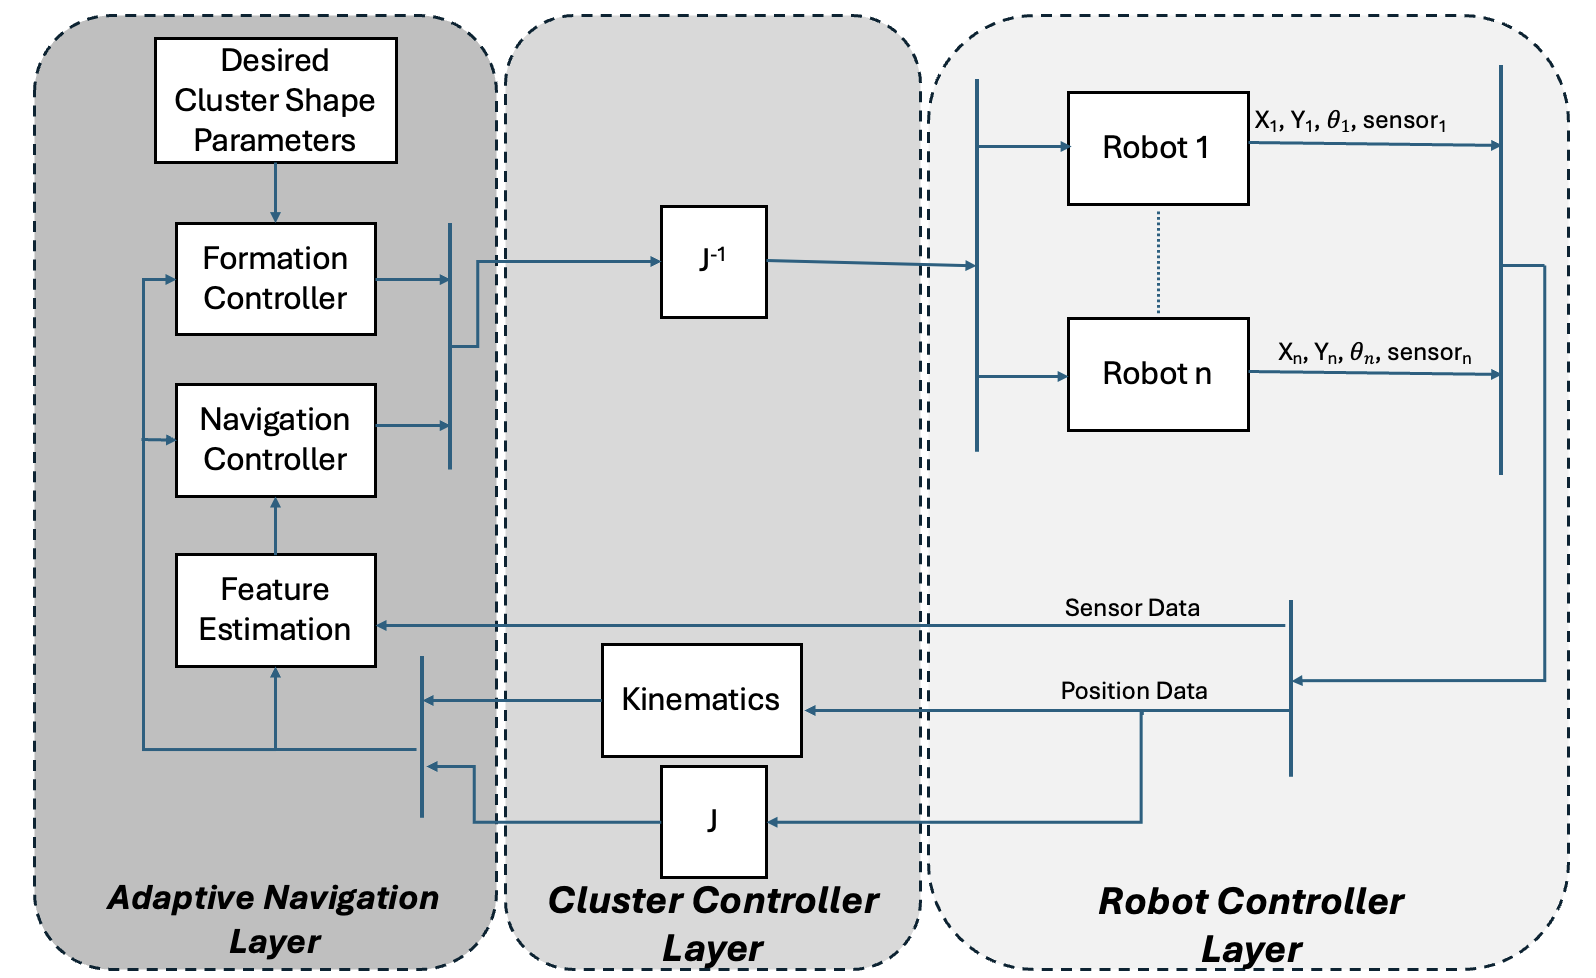
\includegraphics[width=0.40\textwidth]{figures/control_architecture.png}
    \caption{Hierarchical control architecture. Robot controller,
    cluster controller, and adaptive navigation layers.}
    \label{fig:control_architecture}
\end{figure}


\subsection{The $D$ Tracker}
\label{sec:sep_controller}

The $D$ tracker drives the cluster centroid onto the trench of $D$ and
then along it, following the separatrix through the crest that separates
one saddle from the next. This is Problem 1. Both motions are built from
the local quadratic surface the estimator returns.

The derivation works in the eigenbasis of the estimated Hessian. Let
$\hat{\mathbf{H}}_{D,0}\mathbf{w}_k = \lambda_k \mathbf{w}_k$ with
$\|\mathbf{w}_k\| = 1$ and $\lambda_1 \leq \lambda_2$. A trench of $D$ is
convex across and concave along, so it is the case
$\lambda_1 < 0 < \lambda_2$. The eigenvector $\mathbf{w}_2$ points across
the trench and $\mathbf{w}_1$ points along it. The sign of an eigenvector
is arbitrary, and the sign of $\mathbf{w}_1$ is fixed so that
$\hat{\mathbf{v}}_0^\top \mathbf{w}_1 \geq 0$, which orients it
downstream.

Because $\hat{D}$ is an exact quadratic surface, the Newton step
$-\hat{\mathbf{H}}_{D,0}^{-1}\hat{\mathbf{g}}_0$ moves in one stroke to
its stationary point. Two properties prevent it from being issued
directly as a velocity command. The first is dimensional. Under the local
quadratic model $\hat{\mathbf{g}}_0 \approx \hat{\mathbf{H}}_{D,0}
\mathbf{r}$, dividing the gradient projection by the curvature cancels
that curvature and leaves $\mathbf{w}_k^\top \mathbf{r}$, a displacement,
so commanding the step as a velocity asks the cluster to close the whole
remaining distance in one unit of time. That demand exceeds the available
speed at any appreciable distance from the structure, and it diverges as
$\hat{\mathbf{H}}_{D,0}$ approaches singularity. The second is geometric.
The stationary point the step seeks is the crest of the trench rather
than a point on the separatrix.

The first is bounded with the hyperbolic saturation
\begin{equation}
    \mathrm{sat}(c) = c_{\max} \tanh\!\left(\frac{c}{c_{\max}}\right),
    \label{eq:sat}
\end{equation}
chosen over a hard clip for its behavior in the two limits. For $|c| \gg
c_{\max}$ the command is a bounded transit at the fixed speed $c_{\max}$,
set neither by the distance to the structure nor by the conditioning of
$\hat{\mathbf{H}}_{D,0}$. For $|c| \ll c_{\max}$ it is transparent,
$\mathrm{sat}(c) \to c$. One parameter therefore fixes both
the transit speed far from the structure and the width of the terminal
boundary layer near it, and no per-eigendirection gains are needed.

The second property is addressed by treating the two eigendirections
separately. Across the trench, the Newton component is the one required
and is kept. Along the trench, its magnitude is kept and its direction
is taken from the ambient flow.

The along-trench command changes character once the cluster reaches the
separatrix. Away from it, the along-trench gradient supplies a descent
rate. On it, that gradient vanishes at the crest and the descent rate
vanishes with it, while the separatrix continues through, so the flow
supplies the speed instead. The cluster is declared on the separatrix,
written $\mathbf{p}_c \in \mathcal{B}$, when
\begin{equation}
    |\hat{D}_0| < \varepsilon_{\mathrm{raw}}
    \quad\text{or}\quad
    \frac{|\hat{D}_0|}{\|\hat{\mathbf{H}}_{D,0}\|_F}
        < \varepsilon_{\dim}.
    \label{eq:flow_band}
\end{equation}
The first test is a raw threshold on the estimated determinant. The
second normalizes it by the local curvature, a ratio with units of length
squared, so the band scales with the landscape rather than with the
absolute size of $D$. The along-trench speed is then
\begin{equation}
    v_\parallel =
    \begin{cases}
        \hat{\mathbf{v}}_0^\top \mathbf{w}_1,
            & \mathbf{p}_c \in \mathcal{B}, \\[6pt]
        \dfrac{|\mathbf{w}_1^\top \hat{\mathbf{g}}_0|}{|\lambda_1|},
            & \text{otherwise},
    \end{cases}
    \label{eq:vpar}
\end{equation}
and the velocity command is
\begin{equation}
    \dot{\mathbf{p}}_c =
    \mathrm{sat}(v_\parallel)\,\mathbf{w}_1
    + \mathrm{sat}\!\left(-\frac{\mathbf{w}_2^\top
      \hat{\mathbf{g}}_0}{\lambda_2}\right)\mathbf{w}_2.
    \label{eq:d_law}
\end{equation}

The two channels are independent. The $\mathbf{w}_2$ term is unaffected
by (\ref{eq:vpar}), so it is the same command on and off the band, and
inside the boundary layer of (\ref{eq:sat}) it is the exact Newton
component with its superlinear local convergence. Since $v_\parallel \geq
0$ in both branches, the tangential motion is never directed against the
ambient flow. Neither term depends on the arbitrary sign of an
eigenvector, the transverse one because it is quadratic in
$\mathbf{w}_2$ and the tangential one because the sign of $\mathbf{w}_1$
is fixed above.

One guard falls outside (\ref{eq:d_law}).
The trench frame is undefined when $\hat{\mathbf{H}}_{D,0}$ has
eigenvalues of one sign, so the law needs a fallback there. Off the
band it reverts to the signed Newton step $\sum_k
\mathrm{sat}(-\mathbf{w}_k^\top\hat{\mathbf{g}}_0/\lambda_k)\mathbf{w}_k$,
which drives the centroid toward the nearest stationary point of
$\hat{D}$ without a stability claim, and on the band it reverts to the
saturated flow alone. With exact estimates, neither case arises on a
trench away from the band boundary.




\subsection{The $s_1$ Tracker}
\label{sec:oecs_controller}


This controller traverses the trench of $s_1$ using four quantities the
fit delivers, the eigenvalue $\hat{s}_1$, its gradient
$\nabla\hat{s}_1$, the strain eigenframe $(\mathbf{e}_1, \mathbf{e}_2)$,
and the deviatoric strain magnitude $r$, which measures how well resolved
that eigenframe is. Remark~\ref{rem:s1hess} rules out a Newton snap on
$s_1$, so both
channels of this controller are built from the gradient rather than the
curvature.

The first step is to identify the trench tangent. Naming an eigenvector
directly will not work, for the reason given in
Section~\ref{sec:strain_field}. The gradient is used instead. On the
trench, the transverse derivative of $s_1$ vanishes by construction, so
away from a stationary point $\nabla\hat{s}_1$ points almost entirely
along the trench, and the tangent is whichever eigenvector the gradient
is less orthogonal to.
\begin{equation}
    \mathbf{t}_{\mathrm{raw}} =
    \arg\max_{\mathbf{e} \in \{\mathbf{e}_1, \mathbf{e}_2\}}
    \bigl\lvert \nabla\hat{s}_1^\top \mathbf{e} \bigr\rvert,
    \qquad
    \mathbf{t} = \mathrm{sgn}\bigl(\mathbf{t}_{\mathrm{ref}}^\top
    \mathbf{t}_{\mathrm{raw}}\bigr)\,\mathbf{t}_{\mathrm{raw}},
    \label{eq:tangent_select}
\end{equation}
where $\mathbf{t}_{\mathrm{ref}}$ is the previous step's tangent once one
has been established, or the measured flow $\hat{\mathbf{v}}_0$ on the
first tracking step. The rule selects $\mathbf{e}_2$ on the attracting
half of the separatrix and $\mathbf{e}_1$ on the repelling half, swapping
automatically through the origin. Continuity fixes only the residual
sign, not the direction.

The controller alternates between traversing and settling, selected by a
ride flag $\beta \in \{0,1\}$ that is one while traversing. The velocity
command is
\begin{equation}
    \dot{\mathbf{p}}_c =
    \beta\,c_{\max}\tanh(1)\,\mathbf{t}
    - \mathrm{sat}\!\bigl(g_\perp\,\mathbf{P}\,\nabla\hat{s}_1\bigr),
    \qquad
    \mathbf{P} = \mathbf{I} - \beta\,\mathbf{t}\mathbf{t}^\top,
    \label{eq:oecs_law}
\end{equation}
where $\mathrm{sat}$ acts on a vector by saturating its magnitude and
preserving its direction, reducing to (\ref{eq:sat}) on any scalar
multiple of a unit vector.

This control law decouples descent from travel through the projector.
With $\beta = 1$, $\mathbf{P}$ removes the along-trench component of the
gradient, so the team descends only across the trench while riding along
it at cruise speed $c_{\max}\tanh(1)$. With $\beta = 0$, the projector
becomes the identity, the ride term drops out, and the same expression
is full gradient descent on $\hat{s}_1$, which settles at a local
minimum. The gain $g_\perp$ is fixed, standing in for the curvature
normalization that Remark~\ref{rem:s1hess} rules out, so the transverse
channel contracts at gradient rate rather than at Newton rate. This is
the cost of objectivity, priced in Section~\ref{sec:objectivity_tradeoff}.
Both channels read the same two projections from
(\ref{eq:tangent_select}), so no additional estimated quantity enters the
ride.

Two situations clear the ride flag. Before the team has reached any
structure, $\beta = 0$ and the descent term homes onto the trench from
anywhere in the basin. First contact is declared, and $\beta$ latches to
one, when $\hat{s}_1$ first falls below $-s_{\mathrm{trim}}$. The second
situation is the terminal behavior, and it holds the team at a
two-dimensional stationary point of $\hat{s}_1$ when
\begin{equation}
    r > r_{\mathrm{band}}, \qquad
    \lVert\nabla\hat{s}_1\rVert < g_{\mathrm{capture}}, \qquad
    \hat{s}_1 < -4 s_{\mathrm{trim}}.
    \label{eq:capture_test}
\end{equation}

A flow saddle is not merely a crossing of two transverse trenches. It is
a genuine two-dimensional minimum of $s_1$, verified numerically at the
double-gyre saddle, so the full gradient collapses there, while at an
ordinary trench point the gradient remains large along the trench even
though it vanishes across it. Testing the gradient magnitude is
therefore enough to distinguish the two. This matters because the
ambient flow also stagnates at a saddle, which would starve any
flow-based tangent rule of a direction exactly where the ride needs one.
The three tests in (\ref{eq:capture_test}) reject, in order, the
isotropic point, an ordinary trench point, and a shallow flat spot of
$\hat{s}_1$ away from real structure. The $-4s_{\mathrm{trim}}$ depth
threshold is a hysteresis ratio rather than a physical relation. The
condition arms at four times the first-contact depth and releases when
$\hat{s}_1$ rises back above $-s_{\mathrm{trim}}$, so a noise-driven
flicker of the gradient test does not send the team back through the
tangent comparison at the well, while a genuine departure still does.

One guard falls outside (\ref{eq:oecs_law}). If the eigenframe is
degenerate, $r < r_{\mathrm{band}}$, and no previous tangent has been
established, then neither (\ref{eq:tangent_select}) nor continuity
supplies a direction. The command then rides the measured flow,
$\mathbf{t} = \hat{\mathbf{v}}_0/\|\hat{\mathbf{v}}_0\|$, with the
projector set to the identity. Only the first tracking step can reach
this case, and it is the one place in the controller where the ambient
flow enters the command.



\subsection{Stability Properties}
\label{sec:stability}

The analysis is at the navigation level, with the cluster centroid a
kinematic integrator
\begin{equation}
    \dot{\mathbf{p}}_c = k\,\boldsymbol{\delta}(\mathbf{p}_c),
    \label{eq:kinematic_model}
\end{equation}
$\boldsymbol{\delta}$ the right-hand side of the active law,
(\ref{eq:d_law}) or (\ref{eq:oecs_law}), and $k > 0$ the navigation
gain. The layers beneath settle in roughly 0.3~s against transit times
of tens of seconds \cite{9}. Estimates are taken exact, so hats are
dropped.

Let $\Sigma$ be the tracked surrogate, $D$ or $s_1$, in arclength
coordinates $(\ell, n)$ along and across a trench segment $\Gamma$ on a
tube $T_w = \{|n| \leq w\}$, where
\begin{equation}
    \Sigma(\ell, n) = h(\ell)
        + \tfrac{1}{2}\kappa_\perp(\ell)\,n^2,
    \qquad 0 < \underline{\kappa} \leq \kappa_\perp(\ell),
    \label{eq:normal_form}
\end{equation}
with vanishing cross terms. $\Gamma$ is taken invariant under the flow,
with $\lVert\mathbf{v}\rVert \geq f_{\min} > 0$ outside balls of radius
$r_0$ around the flow saddles, and $|h'(\ell)| \geq m_h > 0$ wherever
the band test fails on $\Gamma$. The transverse gradient $\kappa_\perp
n$ vanishes on $\Gamma$ and nowhere else in the tube, so the problem
splits, regulate $n$ to zero and transport along $\ell$.

Both controllers command the same transverse law
\begin{equation}
    \dot{n} = -c_{\max}\tanh\!\left(
        \frac{a_\perp\,n}{c_{\max}}\right),
    \label{eq:n_dynamics}
\end{equation}
and differ only in the transverse rate $a_\perp$. The $D$ tracker
normalizes by the estimated curvature, giving the Newton argument
$-\kappa_\perp n/\kappa_\perp = -n$ and a fixed $a_{\perp,D} = 1$. The
$s_1$ tracker has no usable curvature (Remark~\ref{rem:s1hess}), so its
rate is set by the field, $a_{\perp,s_1} = g_\perp\,\kappa_\perp(\ell)$.
With $V = \tfrac{1}{2}n^2$, $\dot{V} = -c_{\max}\,n\tanh(a_\perp
n/c_{\max}) < 0$ for $n \neq 0$, so $T_w$ is forward invariant, the
proportional region $|n| < c_{\max}/a_\perp$ is entered in finite time,
and inside it $\dot{V} \leq -2a_\perp\tanh(1)V$.

\begin{theorem}[Network traversal]
\label{thm:separatrix}
Under (\ref{eq:normal_form}) and the flow conditions above, with exact
estimates, every
trajectory starting in $T_w$ (i) remains in $T_w$ and converges
exponentially to $\Gamma$, and (ii) traverses $\Gamma$ in the direction
of the ambient flow, reaching the $r_0$ neighborhood of a flow saddle in
finite time bounded by $L_\Gamma/m$, with $L_\Gamma$ the length of
$\Gamma$ and $m > 0$ the realized tangential speed.
\end{theorem}

\begin{IEEEproof}
Part (i) is the transverse argument above, which holds in both branches
of (\ref{eq:vpar}) since neither transverse command contains $v_\parallel$, the
exponential rate following from concavity of $\tanh$. For (ii), both
branches return $v_\parallel \geq 0$ with $\mathbf{w}_1$ signed so that
$\hat{\mathbf{v}}_0^\top\mathbf{w}_1 \geq 0$, and each is bounded below,
by $f_{\min}$ on the band and by $m_h/\bar{\lambda}_\parallel$ off it,
with $\bar{\lambda}_\parallel$ bounding $|\lambda_1|$ on the tube. Since
$\tanh$ is increasing, the realized tangential speed is at least
\begin{equation}
    m = c_{\max}\min\bigl\{\tanh(f_{\min}/c_{\max}),\;
    \tanh(m_h/\bar{\lambda}_\parallel c_{\max})\bigr\},
    \label{eq:progress_rate}
\end{equation}
and (i) holds in both branches, so the band test cannot reverse $\ell$
and a trench of length $L_\Gamma$ takes at most $L_\Gamma/m$.
\end{IEEEproof}

The trackers end differently at a saddle. There $D$ has a local minimum
with $\mathbf{H}_D \succ 0$ and the degenerate case of (\ref{eq:d_law})
is active, but the floor $e$ of Section~\ref{sec:sensitivity} leaves the
estimated eigenvalues indefinite even without noise, so the $D$ tracker
rides onto the crossing segment and repeats (i) and (ii) with $\Gamma$
relabeled. The $s_1$ tracker stops. Once the ride flag clears, the
projector is the identity, (\ref{eq:oecs_law}) is gradient descent on
the surrogate itself, and $\dot{s}_1 \leq 0$ with equality only at a
critical point. That is the vanishing-gradient test
Section~\ref{sec:sensitivity} admits rather than the definiteness test it does
not.

Estimation error, and any residual cross term $\kappa_\perp'(\ell)\,n$,
enters the transverse channel as a bounded disturbance $|d| \leq
\delta$. Then $\dot{V} < 0$ outside an interval and the structure is
practically stable, with
\begin{equation}
    \limsup_{t\to\infty}|n(t)| \;\leq\;
    \frac{c_{\max}}{a_\perp}
    \operatorname{artanh}\!\left(\frac{\delta}{c_{\max}}\right)
    \;\approx\; \frac{\delta}{a_\perp},
    \label{eq:iss_bound}
\end{equation}
for $\delta \ll c_{\max}$, the disturbance divided by the local slope of
the restoring law. Here
$\delta$ is the transverse gradient error, placed at
$\nu/\tilde{\rho}^{\,2}$ by (\ref{eq:error_budget}), so tracking error
degrades linearly in measurement noise.

Two bandwidth limits sit underneath this, and both read off $a_\perp$
alone. Explicit Euler at step $\Delta t$ makes the near-structure map $n
\mapsto n(1 - \Delta t\,k\,a_\perp)$, monotone below $\Delta t\,k\,
a_\perp = 1$ and stable below $2$, and the kinematic abstraction
separately needs $k\,a_\perp\tau \ll 1$. A rate fixed by
design meets both through the choice of $k$, and a rate set by the field
does not.

\begin{proposition}[Frame equivariance of the closed loop]
\label{prop:equivariance}
Let an observer rotate as $\mathbf{p}_Q = \mathbf{Q}(t)\mathbf{p}$ and
let the $s_1$ tracker run with exact estimates on the correspondingly
transformed field. Then $\boldsymbol{\delta}_Q =
\mathbf{Q}\boldsymbol{\delta}$ and $\mathbf{p}_{c,Q}(t) =
\mathbf{Q}(t)\mathbf{p}_c(t)$ up to the frame-transport term, so the
tracker follows the same material path in every frame. The single
exception is the degenerate guard, reachable only on the first tracking
step.
\end{proposition}

\begin{IEEEproof}
By Section~\ref{sec:strain_field} the transport term in $\mathbf{J}_Q$ lands in the
spin part, so $\mathbf{S}_Q = \mathbf{Q}\mathbf{S}\mathbf{Q}^\top$,
leaving $s_1$ and $r$ invariant and the eigenframe and $\nabla s_1$
co-rotating. Every test in (\ref{eq:oecs_law}) and
(\ref{eq:tangent_select}) is a scalar inequality in those invariants, so
the tangent is equivariant by induction from the second tracking step
onward and $\boldsymbol{\delta}_Q = \mathbf{Q}\boldsymbol{\delta}$
follows on integrating (\ref{eq:kinematic_model}). The degenerate guard
is the exception. It reads the measured flow, carrying
$\dot{\mathbf{Q}}\mathbf{Q}^\top\mathbf{p}_Q$ with no inertial
counterpart, and is reachable only on the first tracking step, before
continuity takes over.
\end{IEEEproof}

The $D$ tracker admits no counterpart, since its surrogate carries the
$O(\mathrm{Ro})$ term of (\ref{eq:rossby}) into everything its law
reads.

\section{Simulation Program}
\label{sec:methods}

\subsection{Simulation Setup}
\label{sec:sim_setup}

A Python simulation implementing the three-layer architecture of
Section~\ref{sec:arch} was developed to evaluate both trackers.
The double-gyre experiments use the steady field of
Section~\ref{sec:dg_example} ($A = 0.1$) on the domain $[-1, 1] \times
[-0.5, 0.5]$. The integrator is explicit Euler at 10~Hz ($\Delta t =
0.1$~s), robot dynamics follow the first-order model
(\ref{eq:momentum}), and the cluster layer distributes the centroid
command to the six robots through the analytic $12 \times 12$ inverse
Jacobian while driving each of the nine formation shape terms to its
nominal value proportionally (gain 1.0 on lengths, 0.1 on angles, fixed
across all experiments). All trials use the nominal formation with ring
radius $\rho = 0.075$; a trial varies only the formation's initial
heading, drawn uniformly from $[0, 2\pi)$ in the Monte Carlo sweeps and
zero in the noise-free demonstration runs. Clean trials run 400 to 600
steps and stop at domain exit or, for the $D$ tracker, 150 steps after
first saddle contact. Noise-sweep trials run up to 500 steps and stop
at task completion or domain exit. The estimator-accuracy sweep holds
the formation static and draws independent noise per trial. It is read
on log--log axes, where the exponents of (\ref{eq:error_budget}) appear
directly as slopes.

\subsection{Robot Model and Gains}
\label{sec:robot_model}

Discretizing (\ref{eq:robot_first_order}) at control period $\Delta t$
gives the momentum model identified on the Decabot hardware, a
six-robot indoor omnidirectional testbed built for this line of work
\cite{39,40}, in \cite{9},
\begin{equation}
    \mathbf{v}[k+1] = \alpha_{\text{mom}}\,\mathbf{v}[k]
    + (1 - \alpha_{\text{mom}})\,\mathbf{v}^{\text{des}}[k],
    \label{eq:momentum}
\end{equation}
where $\alpha_{\text{mom}} = e^{-\Delta t/\tau}$ is the momentum
coefficient (Table~\ref{tab:params}), giving $\tau = -\Delta
t/\ln\alpha_{\text{mom}} \approx 0.28$~s at $\Delta t = 0.1$~s,
consistent with the identified Decabot lag. Each robot also carries a
speed limit and a stiction floor.
The trackers saturate every command channel through
$c_{\max}\tanh(c/c_{\max})$, so the commanded centroid speed never
exceeds $\sqrt{2}\,c_{\max}$. The primitive command is amplified by a
fixed navigation gain $k$ so that steady commands clear the stiction
floor. Table~\ref{tab:params} collects all robot and controller
parameters, fixed across every experiment unless noted. The double-gyre
core wells have depth $s_1 = -\pi^2 A \approx -0.987$, well past
$-4s_{\mathrm{trim}}$ for the values in the table.

\begin{table}[!t]
\centering
\caption{Simulation and controller parameters at the two operating
points, laboratory Decabot (double gyre) and ocean HFR
(Section~\ref{sec:ocean_sim}). Ocean values are in world units per simulated
step; the Ocean (phys.) column applies the conversions of
Section~\ref{sec:ocean_sim}.}
\label{tab:params}
\scriptsize
\setlength{\tabcolsep}{2.5pt}
\begin{tabular}{@{}lccc>{\raggedright\arraybackslash}p{0.30\linewidth}@{}}
\hline
\textbf{Sym.} & \textbf{Decabot} & \textbf{Ocean} & \textbf{Ocean (phys.)} & \textbf{Description} \\
\hline
$c_{\max}$ & 0.04 & 0.04 & 3.4~m/s & primitive saturation speed \\
$k$ & 3.0 & 1.8 & --- & navigation gain \\
$v_{\text{max,robot}}$ & 0.3 & 0.3 & --- & robot speed limit \\
$v_{\text{stiction}}$ & 0.025 & 0.002 & --- & stiction floor \\
$\alpha_{\text{mom}}$ & 0.7 & 0 & --- & momentum coefficient \\
$\rho$ & 0.075 & 0.105 ($1.4\times$) & 5.4~km & formation ring radius \\
$\varepsilon_{\text{raw}}$ & $10^{-3}$ & $10^{-3}$ & --- & on-structure raw thr. \\
$\varepsilon_{\text{dim}}$ & 0.025 & 0.025 & --- & on-structure curv.-norm. thr. \\
$g_\perp$ & 1.0 & 1.0 & --- & $s_1$-descent gain \\
$s_{\text{trim}}$ & 0.05 & 0.3 & --- & first-contact threshold \\
$g_{\text{capture}}$ & 0.15 & 0.15 & --- & terminal gradient-mag. thr. \\
$r_{\text{band}}$ & 0.05 & 0.05 & --- & eigenframe-resolution thr. \\
\hline
\end{tabular}
\end{table}

\subsection{Ocean HFR Setup}
\label{sec:ocean_sim}

The ocean experiment uses hourly surface-current frames for the Santa
Barbara Channel from the HFRNet U.S.~West~Coast Radial-to-Total Vector
product \cite{41}, on the $2$~km grid. The record is the same one
\cite{17} uses for its own Santa Barbara Channel experiment, the same
network over the same 28-h window, 29 frames from May 16, 2012 08:00
GMT to May 17, 2012 12:00 GMT, so the two methods are directly
comparable on the same data. Frames are interpolated linearly in time
inside the field evaluator. World coordinates on $[-0.65, 0.65]^2$ map
affinely onto a region of radius $0.3^{\circ}$ centered on
$(34.2^{\circ}\mathrm{N}, -120.4^{\circ}\mathrm{W})$, so one world unit
is approximately $51$~km and one simulated step represents $600$~s of
field time. The $168$-step trial spans the full record.

The Ocean column of Table~\ref{tab:params} gives the resulting
operating point. The pentagon is enlarged to $\rho = 0.105$,
$1.4\times$ the nominal radius and $5.4$~km at this site, so the
six-robot footprint spans about five cells of the $2$~km grid rather
than under four. At one control cycle per ten minutes any vessel time
constant is negligible, so $\alpha_{\text{mom}} = 0$, and the stiction
floor drops to $0.002$, a motor-friction floor with no vessel-scale
analogue. The navigation gain $k = 1.8$ follows the ridge branch that
makes landfall on the middle island, at a realized mean speed near
$0.5$~m/s, well inside the commanded cap. No noise level is estimated
for this field. The exactly-determined six-robot fit leaves no residual
to estimate $\sigma_{uv}$ from, and quantifying the uncertainty in
actual ocean data and its impact on the proposed tracking strategy is,
in the words of \cite{17} on this same record, ``extremely challenging
and outside the scope.'' The noise model of Section~\ref{sec:test_plan} is
validated on the double gyre only.

\subsection{Test Plan}
\label{sec:test_plan}

Four experiment families validate the trackers, alongside three
supporting checks.

\subsubsection{Double-gyre clean runs}
Each tracker runs noise-free from the same six initial conditions,
spanning both gyre halves, the origin, and points off the structure
entirely, checked against the analytic geometry of Section~\ref{sec:dg_example}. Each
run records the step at which the
centroid first reaches the trench and holds it, the closest approach to
each saddle, and whether the run settles at a saddle or continues
through it onto the crossing wall trench. Running both trackers from
identical starts also gives the pairwise path gap between them, the mean
nearest-point distance over the portion of the run where both are on the
structure. The $s_1$ tracker's terminal test (\ref{eq:capture_test}) is
unconditional by design and fires without a separate setting to enable it.

\subsubsection{Monte Carlo noise sweeps}
Both trackers sweep the same two-dimensional noise grid from one
straddling start, $(0, 0.35)$, so the success rate measures noise
robustness rather than basin geometry. The grid spans $\sigma_{uv} \in
\{0,\, 0.001,\, 0.005,\, 0.01,\, 0.02,\, 0.05,\, 0.1\}$, with the top
level doubled and re-swept up to three times while the worst cell still
succeeds above 10\% ($\sigma_{uv} = 0.8$), and $\sigma_p \in \{0,\,
0.005,\, 0.01,\, 0.02,\, 0.05\}$, at 10\,000 trials per cell of at most
500 steps, each from an independent initial heading. Success is contact
within 0.06 of the far saddle $\mathbf{p}^*_1 = (0, -0.5)$, which a
noise-free run from this start reaches under either law, without
formation collapse (root-mean-square error of the fifteen inter-robot
distances from nominal above 0.30, four times $\rho$). Holding one
target fixed for both surrogates makes a settle at the near saddle a
directional failure rather than a loss of the structure, and each trial
records which saddle it settles at. Each trial also records straddle
retention (robots on both sides of the separatrix from first
straddle to stop, the failure count of \cite{17}, used here as an
internal metric only) and tracking error (mean and 95th percentile of
$|x_c|$). The $s_1$ sweep widens the exit box to
$|y| \leq 0.60$ against $0.52$, for the few-centimeter terminal
overshoot of (\ref{eq:oecs_law}); step budget, start, contact radius,
and collapse guard are identical. Its transition is resolved on each
noise axis separately at 0.0005 spacing
(Fig.~\ref{fig:flip_resolution}).

\subsubsection{Objectivity demonstration}
Both trackers run from $(0.05, 0.40)$, just inside the upper saddle, on
the same physical double gyre expressed in two
observer frames, the inertial frame, and a frame rotating at
$\Omega = 0.2$ rad/s, in which the field is
$\mathbf{v}'(\mathbf{p}', t) = \mathbf{Q}\mathbf{v}(\mathbf{Q}^\top
\mathbf{p}') + \Omega\,(-y', x')^\top$. The added solid-body vorticity
$2\Omega = 0.4$ is 20\% of the gyre-core vorticity. The rate keeps the
structure's apparent speed at the tracked radius, $\Omega r \leq 0.10$,
inside the command authority $k\,c_{\max} = 0.12$. Rotating-frame
trajectories are pulled back to inertial coordinates and compared with
the inertial run of the same tracker, both by their final separation and
by each run's mean distance to the true trench network.
Proposition~\ref{prop:equivariance} predicts near-zero gaps for the
$s_1$ tracker and offers no such protection to the $D$ tracker, whose
surrogate obeys (\ref{eq:D_not_objective}).

\subsubsection{Ocean runs}
Both trackers run unmodified, from a single shared start, on the Santa
Barbara Channel field at the Ocean operating point of
Table~\ref{tab:params}, evaluated against the 24-h forward-time FTLE
field computed offline from the full radar grid. A $10 \times 10$ grid
of jittered starts tests start sensitivity for the $D$ tracker.

\subsubsection{Supporting checks}
Three checks sit alongside the four families. The estimator-accuracy
sweep of Section~\ref{sec:sim_setup} draws $10^4$ realizations per condition at a
fixed strain-region point, and at the nominal radius the fitted shear
strain, the $\hat{\mathbf{H}}_{s_1}$ eigenvalues, the transverse
component of (\ref{eq:grad_s1}), and the direction error of
$\mathbf{e}_2$ are compared against their analytic values. The clean
runs are repeated over $r_{\text{band}}$ from 0.05 to 0, to test whether
the degenerate-frame guard is needed at the isotropic point. Finally,
acquisition is swept over the same $\sigma_{uv}$ grid at $\sigma_p \in
\{0, 0.01\}$, 1000 trials per cell, from two clean-run starts $2.7\rho$
off the structure, scored on closest approach to the trench network
rather than arrival at a saddle.

\section{Results and Discussion}
\label{sec:results}

\subsection{Estimator Accuracy}
\label{sec:results_est}

\begin{figure*}[!t]
    \centering
    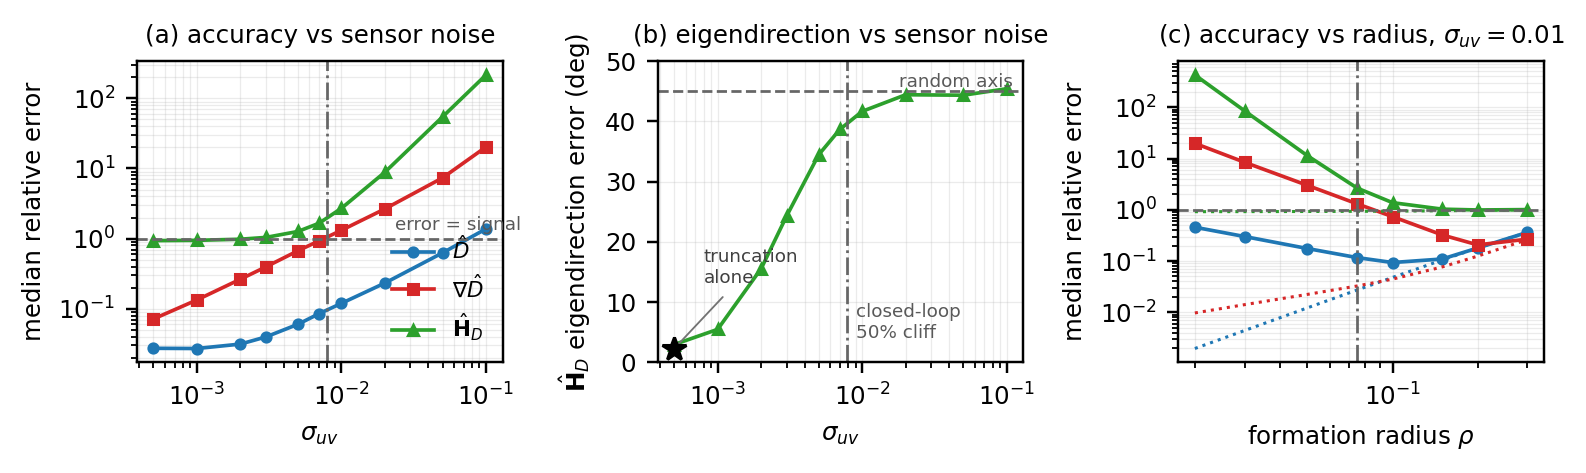
\includegraphics[width=\textwidth]{figures/estimator_accuracy_vs_noise.png}
    \caption{Estimator accuracy on the steady double gyre at the strain-region
    point $(-0.3, 0.1)$, $10^4$ noise draws per point. (a) Median relative error
    of $\hat{D}$, $\nabla\hat{D}$, and $\hat{\mathbf{H}}_D$ against measurement
    noise at $\rho = 0.075$. The dashed line marks error equal to signal, the
    dash-dotted line the noise at which closed-loop traverse success crosses
    50\% (Table~\ref{tab:mc_success}(a)). (b) Mean angle between the fitted and
    the true principal eigenvector of $\hat{\mathbf{H}}_D$, against the
    $45^\circ$ expected of a uniformly random axis. The star is truncation
    acting alone. (c) The same three errors against formation radius at
    $\sigma_{uv} = 0.01$, with the noise-free truncation floors dotted. On these
    axes the exponents of (\ref{eq:error_budget}) appear as slopes.}
    \label{fig:est_accuracy}
\end{figure*}

The estimator was characterized on the steady double gyre before any loop
was closed, over $10^4$ draws per condition at the strain-region point
$(-0.3, 0.1)$. Every prediction of Section~\ref{sec:sensitivity} held.
Coefficient standard deviations matched (\ref{eq:gain_ladder}) within
2.1\%, the reading error induced by position noise matched
(\ref{eq:sigma_eff}) within 1.6\%, the downward bias of $\hat{s}_1$ matched
(\ref{eq:s1_bias}) within 5\% in eighteen of twenty-four conditions, and
the signed mean error of $\hat{D}$, $\nabla\hat{D}$, and
$\hat{\mathbf{H}}_D$ was zero to within 2.7\% of one standard deviation
across forty-eight conditions, as Proposition~\ref{prop:unbiased} requires.
The correlation between the two component errors at one robot was $0.41$
under position noise against $0.44$ predicted, and zero under measurement
noise, which is the mechanism separating the channels.

In Fig.~\ref{fig:est_accuracy}(a), $\hat{D}$ stays informative to
$\sigma_{uv} \approx 0.07$ and $\nabla\hat{D}$ to $\approx 0.0075$, while
$\hat{\mathbf{H}}_D$ never falls below the error-equals-signal line at any
noise level, held there by $e$ at every radius in
Fig.~\ref{fig:est_accuracy}(c). In Fig.~\ref{fig:est_accuracy}(b),
truncation acting alone costs the $\hat{\mathbf{H}}_D$ eigendirections
$2.2^\circ$, while noise costs them $24^\circ$ by $\sigma_{uv} = 0.003$ and
$39^\circ$ at the closed-loop failure cliff below, against $45^\circ$ for a
uniformly random axis.

The $s_1$ channel was checked at the nominal radius against its analytic
values. The fitted shear strain at three test points is at the $10^{-4}$
level (analytic value zero), and the fitted $\hat{\mathbf{H}}_{s_1}$
eigenvalues are $[-0.011, 0.000]$ and smaller, negative semidefinite as
Remark~\ref{rem:s1hess} requires. The transverse component of
(\ref{eq:grad_s1}) at $(0.03, 0.25)$ recovers the restoring slope $4.0$ per
unit offset against the analytic transverse curvature $6.9$, the two values
entering Table~\ref{tab:bandwidth}. At $\sigma_{uv} = 0.01$ the median
direction error of $\mathbf{e}_2$ is $4.5^\circ$, against $44^\circ$ for
$\nabla\hat{s}_1$ and $41^\circ$ for the $\hat{\mathbf{H}}_D$ eigenvector
($2\times 10^4$ draws per level).

\subsection{Clean Runs}
\label{sec:disc_clean}

\begin{figure}[!t]
    \centering
    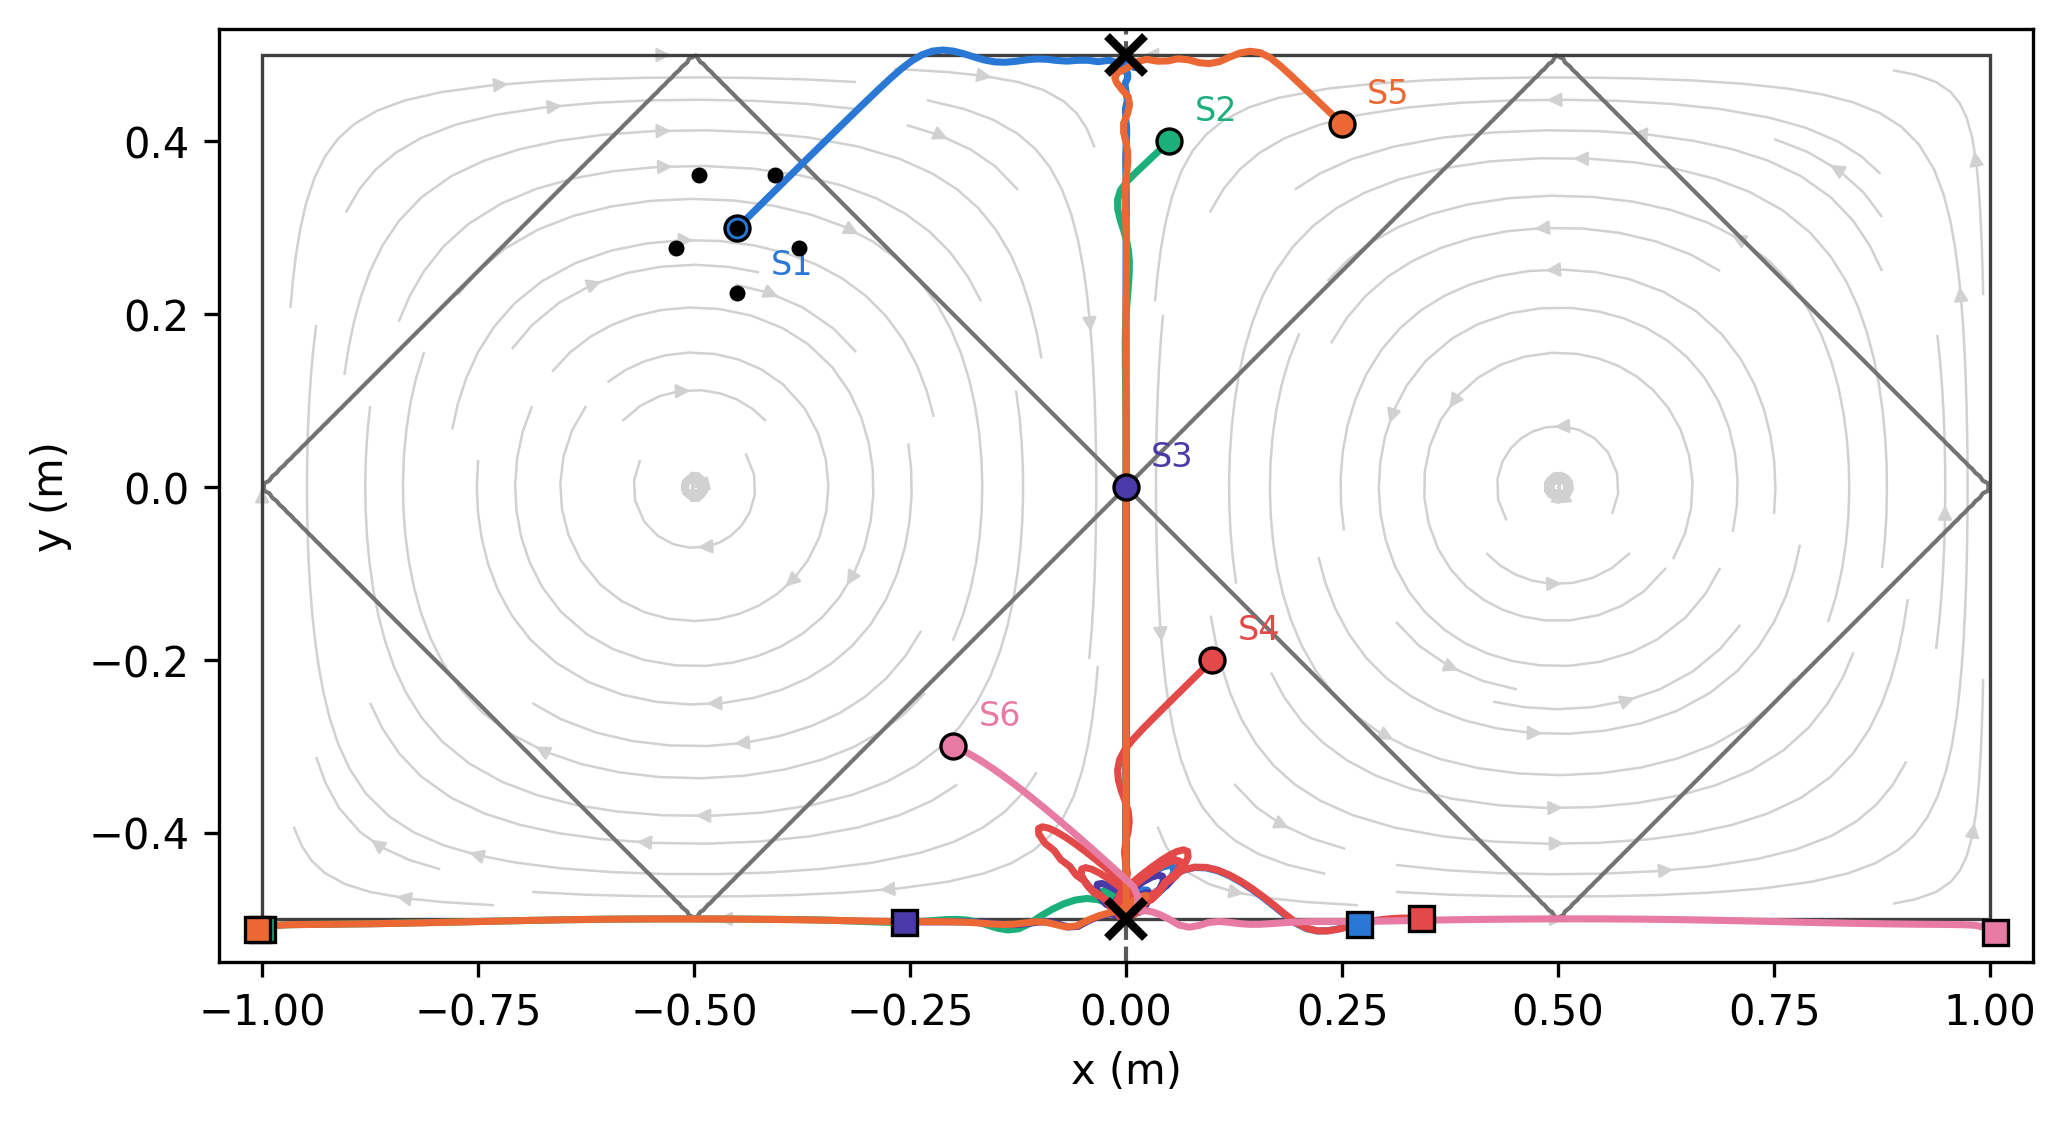
\includegraphics[width=0.34\textwidth]{figures/separatrix_trajectories.png}
    \caption{Noise-free $D$ tracker trajectories from six starts
    ($\bullet$), overlaid on the double-gyre streamlines and Okubo-Weiss
    diamonds. Every run reaches $x = 0$ and continues through the
    terminal saddle ($\times$) along the wall trench, ending at the
    square markers.}
    \label{fig:sep_trajectories}
\end{figure}

\begin{figure}[!t]
    \centering
    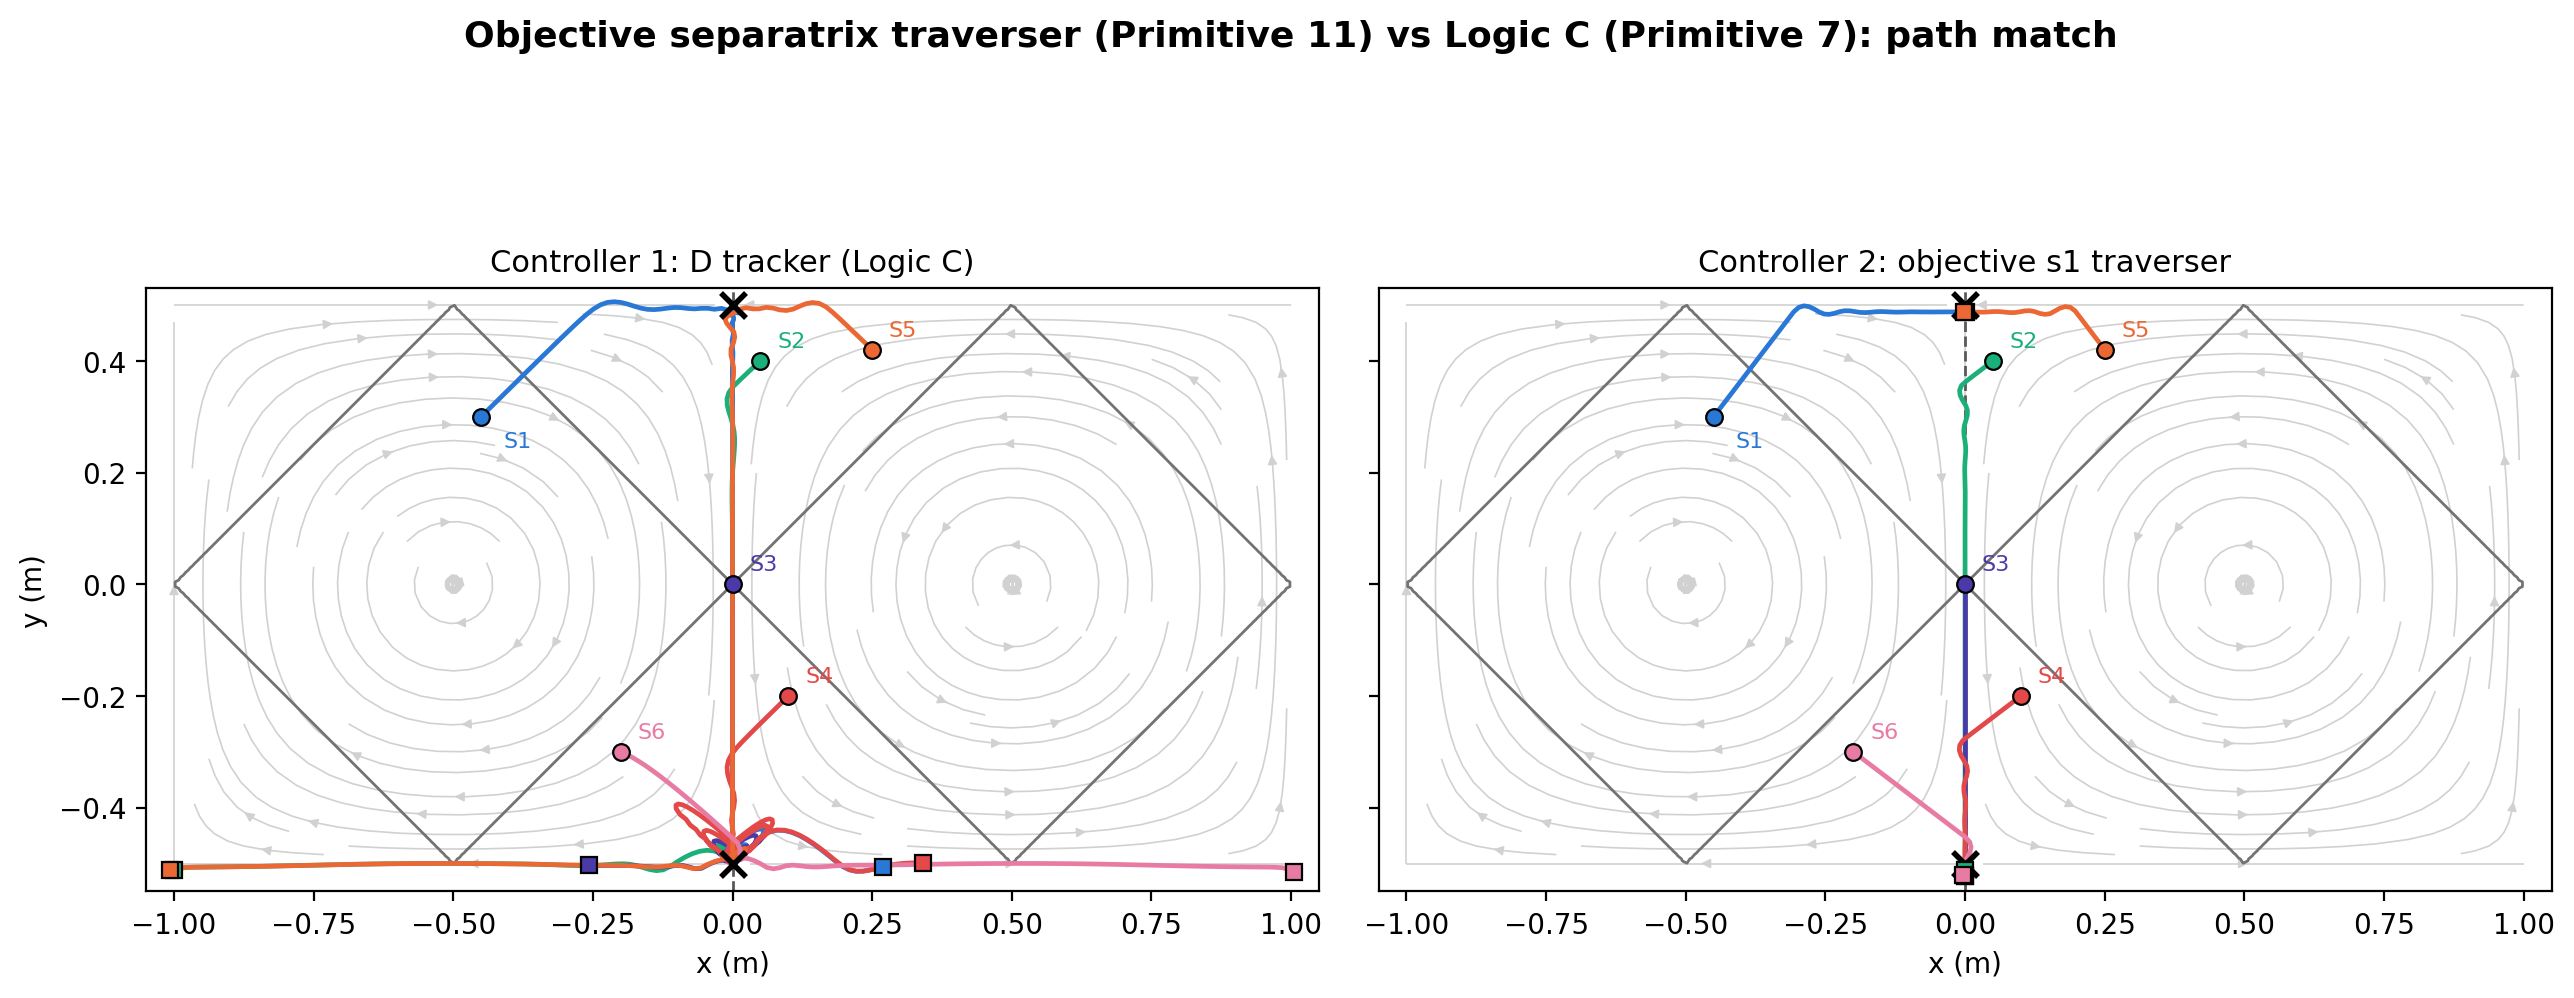
\includegraphics[width=0.34\textwidth]{figures/traverse_vs_logic_c.png}
    \caption{$s_1$ tracker versus $D$ tracker, six matched starts,
    noise-free. Both traverse the same network through the isotropic
    point at the origin. The $s_1$ tracker captures at the saddle its
    tangent orientation resolves toward, while the $D$ tracker
    continues onto the crossing wall trench past every saddle it
    reaches.}
    \label{fig:traverse_vs_logic_c}
\end{figure}

Both trackers were run noise-free from the same six starts
(Fig.~\ref{fig:sep_trajectories}), spanning both gyre halves, the origin,
and points off the structure entirely, between $0$ and $2.7\rho$ from the
nearest trench segment ($\rho = 0.075$, the formation radius). Both acquire
the trench network from every start, in 6 to 35 steps for the $D$ tracker
and 0 to 46 for the $s_1$ tracker, then ride the same segments in the same
direction and cross the isotropic point at the origin.
Theorem~\ref{thm:separatrix} does not distinguish them: the normal form
(\ref{eq:normal_form}) is written for either surrogate and both laws
command the same transverse dynamics (\ref{eq:n_dynamics}). Where the two
commit to the same saddle the paths are visually coincident, and the mean
path gaps of 0.020 to 0.322 over the common on-trench portion
(Fig.~\ref{fig:traverse_vs_logic_c}) open only where they commit to
different ones. Neither needs dedicated machinery at the crossing. The
$s_1$ tracker rides through the origin on ordinary tangent selection
(\ref{eq:tangent_select}), and over the sweep of $r_{\text{band}}$ from
0.05 to 0 the degenerate-frame guard never fires once.

The agreement is exact rather than approximate, and (\ref{eq:splitting})
says why. Differentiating it across the structure gives
\begin{equation}
    \frac{\partial D}{\partial n} =
    \frac{\omega}{2}\frac{\partial \omega}{\partial n}
    - 2 s_1 \frac{\partial s_1}{\partial n},
    \label{eq:trench_coincide}
\end{equation}
so on a curve where the vorticity vanishes, and where the flow is
strain-dominated so that $s_1 < 0$, the two transverse derivatives vanish
together and the two trenches are the same curve. The double gyre's entire
trench network is such a set. With the field (\ref{eq:dg_u}), $\omega =
-2\pi^2 A \sin(\pi x_f)\sin(\pi y_f)$, identically zero on the separatrix
$x_f = 1$ and on all four walls. The lone exception is the isotropic point
at the origin, where $\mathbf{J}$ vanishes entirely and the step from
(\ref{eq:trench_coincide}) is unavailable. The six clean runs therefore
agree pointwise for a reason specific to this field, not because the two
surrogates are interchangeable in general.

The trackers part only at the terminal step, and the split is a fact about
the model class rather than about tuning. The $s_1$ tracker settles within
0.011 to 0.022 of a saddle in every run, at whichever one its initial
tangent orientation resolves toward, four at $\mathbf{p}^*_1 = (0, -0.5)$
and two at $\mathbf{p}^*_2 = (0, 0.5)$. The $D$ tracker passes within 0.02
of $\mathbf{p}^*_1$ (closest approach 0.0003--0.0194), then rides onto the
crossing wall trench and continues, because the capture test
$\lambda_1\lambda_2 \geq 0$ does not fire even without noise. Near the well
the estimated eigenvalues are indefinite and more than an order of
magnitude too small, held there by the floor $e$ on $\hat{\mathbf{H}}_D$
(Section~\ref{sec:sensitivity}), so the definiteness the test asks about is
not a quantity the fit returns. The same limit binds in both directions.
Under a quadratic velocity fit $\hat{\mathbf{H}}_{s_1}$ is negative
semidefinite for every field and every formation
(Remark~\ref{rem:s1hess}), so neither surrogate admits a definiteness
certificate. The one terminal test a quadratic fit does support is a
vanishing gradient, and a flow saddle is a genuine two-dimensional minimum
of $s_1$, so that test is sufficient exactly where the $s_1$ tracker needs
one and unavailable where the $D$ tracker would need one, which makes the
traversal and the capture the same representability limit read twice.

The clean-field descent also fixes the reachable set, and it is not the
Okubo-Weiss partition. No start settles at a gyre core, and descent of
$\hat{D}$ from the rotation-dominated interiors reaches the trench network
within the 500-step horizon in all 20\,000 runs. The reachable set is
instead the watershed of that descent composited with the flow direction on
the acquired branch, whose arrival rate at $\mathbf{p}^*_1$ is 47.4\% over
a grid of starts and 47.1\% over $n = 10{,}000$ uniformly random starts and
headings. Prior adaptive-navigation primitives \cite{3}, \cite{4} report
local convergence without such an estimate.

A spot check on the time-varying field, $\varepsilon = 0.1$ and
$\omega_{dg} = 2\pi/10$ against the static $\varepsilon = 0$ used
everywhere else, runs the $D$ tracker down the oscillating trench at zero
noise. The trench swings $\pm 0.116$ in $x$ with peak speed equal to 62\%
of the commanded speed cap, and the tracker holds it with mean transverse
offset 0.006 and maximum 0.015, with no time-derivative term in the
controller and no analytic guarantee for that case.

\subsection{Behavior Under Noise}
\label{sec:disc_noise}

\begin{table}[!t]
\centering
\caption{Monte Carlo traverse success (\%), 10\,000 trials per cell
from the straddling start $(0, 0.35)$ with a random heading per trial,
for the (a) $D$ and (b) $s_1$ trackers. Both are scored against the
single far saddle $\mathbf{p}^*_1$ a noise-free run from this start
reaches.}
\label{tab:mc_success}
\footnotesize
\setlength{\tabcolsep}{4.5pt}
\begin{tabular}{@{}l|rrrrr@{}}
\hline
& \multicolumn{5}{c}{$\sigma_p$} \\
\cline{2-6}
$\sigma_{uv}$ & 0.000 & 0.005 & 0.010 & 0.020 & 0.050 \\
\hline
\multicolumn{6}{@{}l}{(a) $D$ tracker} \\
0.000 & 100.0 &  65.7 &  44.5 &  33.3 &  19.0 \\
0.001 &  99.6 &  63.2 &  45.6 &  32.9 &  19.1 \\
0.005 &  62.4 &  52.1 &  43.5 &  31.2 &  19.4 \\
0.010 &  43.7 &  40.7 &  37.0 &  28.8 &  18.7 \\
0.020 &  25.5 &  25.7 &  24.3 &  22.6 &  17.0 \\
0.050 &  16.0 &  16.2 &  15.8 &  16.1 &  14.9 \\
0.100 &  14.1 &  14.1 &  14.3 &  14.6 &  13.6 \\
0.200 &  13.5 &  12.4 &  12.8 &  12.8 &  12.4 \\
0.400 &  12.1 &  12.2 &  12.0 &  12.3 &  11.9 \\
0.800 &   4.8 &   5.4 &   5.1 &   5.4 &   5.2 \\
\hline
\multicolumn{6}{@{}l}{(b) $s_1$ tracker} \\
0.000 & 100.0 &   1.3 &   0.0 &   0.0 &   0.0 \\
0.001 &  91.8 &   1.1 &   0.0 &   0.0 &   0.1 \\
0.005 &   0.0 &   0.0 &   0.0 &   0.0 &   0.0 \\
0.010 &   0.0 &   0.0 &   0.0 &   0.0 &   0.0 \\
0.020 &   0.0 &   0.0 &   0.0 &   0.0 &   0.1 \\
0.050 &   0.2 &   0.2 &   0.1 &   0.1 &   0.1 \\
0.100 &   0.5 &   0.4 &   0.4 &   0.4 &   0.3 \\
0.200 &   0.5 &   0.4 &   0.6 &   0.4 &   0.4 \\
0.400 &   0.5 &   0.5 &   0.5 &   0.6 &   0.5 \\
0.800 &   0.5 &   0.7 &   0.4 &   0.6 &   0.5 \\
\hline
\end{tabular}
\end{table}

\begin{figure*}[!t]
    \centering
    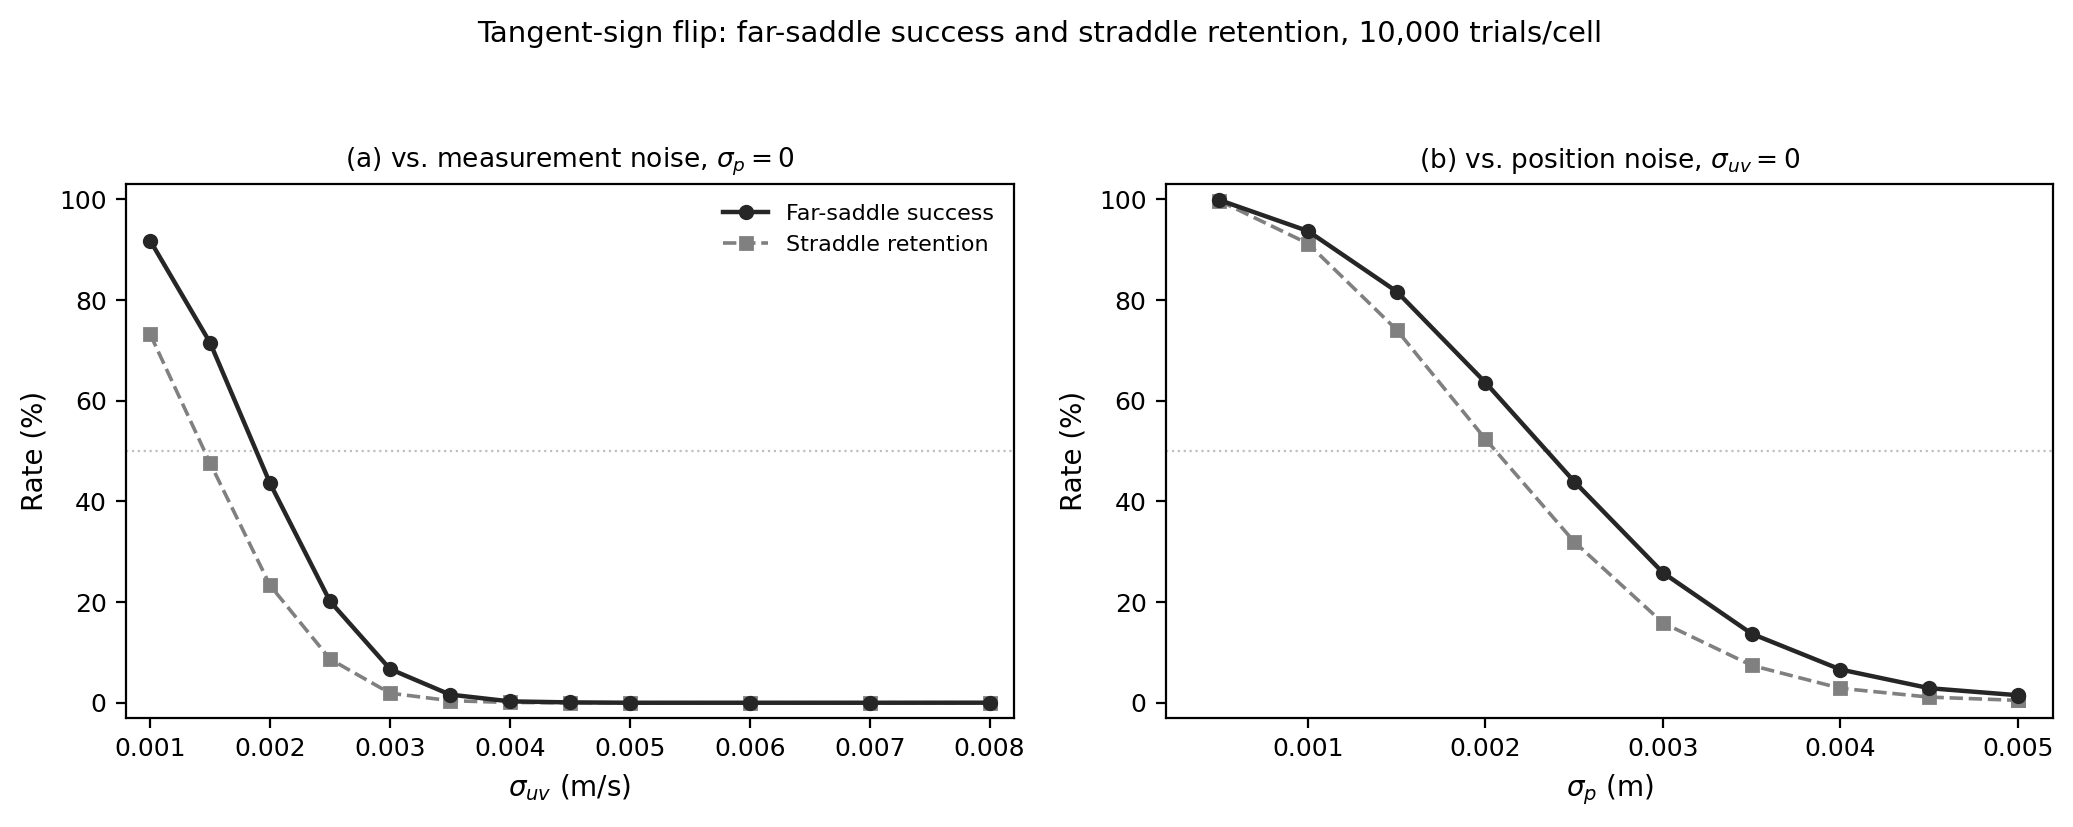
\includegraphics[width=0.78\textwidth]{figures/flip_resolution.png}
    \caption{Resolving the tangent-sign flip. Far-saddle success and
    straddle retention (both conditioned on reaching $\mathbf{p}^*_1$),
    10\,000 trials/cell, at 0.0005 spacing on each axis. (a) Against
    $\sigma_{uv}$, $\sigma_p = 0$. Success crosses 50\% between
    $\sigma_{uv} = 0.0015$ and 0.002 and reaches a sub-1\% floor by
    0.005, held out to 0.008. (b) Against $\sigma_p$, $\sigma_{uv} = 0$.
    The same decline, crossing 50\% between $\sigma_p = 0.002$ and
    0.0025. The transition is resolved and continuous on both axes; what
    is abrupt is the outcome it selects between, since runs on either
    side of it settle at a saddle with comparable reliability and differ
    in which one.}
    \label{fig:flip_resolution}
\end{figure*}

Table~\ref{tab:mc_success} reports traverse success for both trackers over
the noise grid of Section~\ref{sec:test_plan}, scored against
$\mathbf{p}^*_1$. Noise separates the two and it favors the $D$ tracker,
whose 50\% crossing sits a full grid step later, and the two do not fail
the same way.

For the $D$ tracker the cliff and an estimator threshold nearly coincide.
Success holds at 100\% with no noise and crosses 50\% at $\sigma_{uv}
\approx 0.0079$, within 5\% of the $\sigma_{uv} \approx 0.0075$ at which
$\nabla\hat{D}$ stops being informative (Section~\ref{sec:results_est}).
Read alone, that agreement suggests the gradient is what runs out.
Fig.~\ref{fig:est_accuracy}(b) shows it is not the only input that has. At
the cliff the curvature eigenframe is already $39^\circ$ from truth against
$45^\circ$ for a uniformly random axis, and it passed $24^\circ$ by
$\sigma_{uv} = 0.003$, well before. Both terms of (\ref{eq:d_law}) are
built on that frame and normalized by its eigenvalues, so the command
inherits the degradation in full. The mechanism is separate from the floor
$e$, which falls on the eigenvalues and leaves the eigendirections nearly
intact. The directions are resolved instead by the separation of the
eigenvalues against the entry noise (\ref{eq:gain_ladder}) places at
$\nu/\tilde{\rho}^{\,2}$, and once that noise reaches the separation the
recovered frame is uniformly distributed. By the cliff both inputs the law
consumes have failed, and the eigenframe failed first. Neither threshold is
a property of (\ref{eq:d_law}), so the estimator, not the control law, sets
the noise ceiling.

Four further readings sit alongside it. Position noise scales the
estimator-accuracy curve by $\|\mathbf{J}\|$ per (\ref{eq:sigma_eff}), so
$\sigma_p = 0.01$ alone and $\sigma_{uv} = 0.01$ alone give nearly
identical rates. Beyond the cliff success levels off in the low tens of
percent through $\sigma_{uv} = 0.2$ rather than falling to zero, an
unbiased-random-walk floor that decays only at $\sigma_{uv} = 0.8$, while
straddle retention, the failure metric of \cite{17}, decays cleanly with no
such floor (1.000, 0.589, and 0.389 at $\sigma_{uv} = 0$, 0.005, and 0.01).
Acquisition is not the noise-limited phase either. Over the acquisition
sweep of Section~\ref{sec:test_plan} the team reached the trench network,
closest approach under 0.05, in every one of the 20\,000 trials through
$\sigma_{uv} = 0.02$. Binning the 40\,000 trials at $\sigma_{uv} \leq
0.01$, $\sigma_p = 0$ by initial-heading quartile gives 75.9--77.1\%
success per quartile, confirming the isotropy of (\ref{eq:gain_ladder}).

The $s_1$ tracker fails earlier, for a reason that has nothing to do with
estimator accuracy.\footnote{The widened exit box of
Section~\ref{sec:test_plan} recovers 30 of the 54 trials the $D$ tracker's
tighter box would have scored as domain exits at $\sigma_p = 0.005$, all of
which exit at $y \in [0.520, 0.529]$ while still converging.} Its success
falls from 91.8\% at $\sigma_{uv} = 0.001$ through
43.5\% at 0.002 to 0.0\% by 0.005, a floor it holds out to 0.008, where the
$D$ tracker's corresponding column falls only from 62.4\% to 43.7\%. Its
zero-noise tracking error is 0.0075, about five times the $D$ tracker's
0.0016. Fig.~\ref{fig:flip_resolution} resolves the transition at 0.0005
spacing on each noise axis separately, and the two panels are one finding
measured twice rather than two failure modes, since position noise enters
the same comparison through the coupling
$\mathbf{J}(\mathbf{p}_i)\boldsymbol{\xi}_i$ of (\ref{eq:pos_noise}) and
$\|\mathbf{J}\| \approx 1$ at this test point. Straddle retention,
conditioned on the same $\mathbf{p}^*_1$ contact, stays below success at
every level shown, 73.2\% against 91.8\% at $\sigma_{uv} = 0.001$ and
47.6\% against 71.5\% at 0.0015. Runs on either side of the transition
settle at a saddle with comparable reliability and differ in which one. The
team has not lost the structure, become erratic, or collapsed. It rides the
separatrix competently and settles, in the wrong direction. This is a sign
inversion rather than a decay toward chance, and it is what makes the
far-saddle column the score that separates the two outcomes, since a
near-saddle settle is indistinguishable from a success in every other
recorded quantity.

The mechanism is the one-time flow read that seeds
$\mathbf{t}_{\text{ref}}$ on the first tracking step. At this start the
differential flow signal across the six sample points spans about 0.12.
Against peak flow, $\pi A \approx 0.314$, $\sigma_{uv} = 0.002$ is a modest
0.6\%. Against that 0.12 span, the denominator the sign decision actually
consumes, the same noise is 1.7\%, and the second reading is the one that
explains the fragility. It explains its shape as well. Because the noise is
comparable to the signal the decision reads, draws above the threshold
cross it in the same direction rather than half reversing and half not, so
the flip is near-total rather than an even split. Tangent selection itself
is not the source, since it uses only the already-computed gradient
projections and survives past the noise level at which every
gradient-based quantity approaches chance. The fragility is specific to the
sign convention at the seed, a single comparison against the ambient flow.

One prediction of Section~\ref{sec:stability} comes out backwards here, and
the discrepancy locates itself. The ultimate bound (\ref{eq:iss_bound}) is
$\delta/a_\perp$, and $a_{\perp,s_1} > a_{\perp,D}$ at this operating
point, so it predicts the smaller zero-noise tracking error for the $s_1$
tracker. The measurement is the reverse. The ordering matches instead the
discrete stability condition of Table~\ref{tab:bandwidth}, which the $s_1$
tracker crosses over the outer half of the structure. The bound is a
continuous-time statement and the limit that binds at this step size is a
discrete one, so a larger $a_\perp$ tightens the first while violating
the second.

\begin{table}[!t]
\centering
\caption{Discrete-time and actuator conditions of Section~\ref{sec:stability} at
the double-gyre operating point of Table~\ref{tab:params} ($\Delta t =
0.1$, $k = 3.0$, $\tau = 0.28$~s, $g_\perp = 1.0$). For the
$s_1$ tracker $\kappa_\perp$ is the local transverse curvature of the
structure, quoted as recovered by the fit and as computed analytically at
the same point.}
\label{tab:bandwidth}
\footnotesize
\setlength{\tabcolsep}{4pt}
\begin{tabular}{@{}lcccl@{}}
\hline
 & $a_\perp$ & $\Delta t\,k\,a_\perp$ &
 $k\,a_\perp\tau$ & \\
\hline
$D$ tracker & $1.0$ & $0.30$ & $0.84$ & monotone \\
$s_1$, fitted $\kappa_\perp = 4.0$ & $4.0$ & $1.20$ & $3.4$ & oscillatory \\
$s_1$, analytic $\kappa_\perp = 6.9$ & $6.9$ & $2.07$ & $5.8$ & limit cycle \\
\hline
\end{tabular}
\end{table}

The general reading is about commitments rather than accuracy. The
direction the $s_1$ tracker rides is the better estimated of the two
tangent sources by an order of magnitude in angle
(Section~\ref{sec:results_est}), and it is still the less robust tracker
here, because one of its decisions is made once and never revisited. A
perturbation large enough to flip that decision does not degrade the run.
It commits the whole ride to the opposite branch. That is why the
transition is continuous on both noise axes while the outcome it selects
between is not. Robustness is set less by the per-cycle accuracy of what a
law reads than by how many of its commitments are unrevisable.

\subsection{Behavior Under a Rotating Observer}
\label{sec:objectivity_tradeoff}

\begin{figure}[!t]
    \centering
    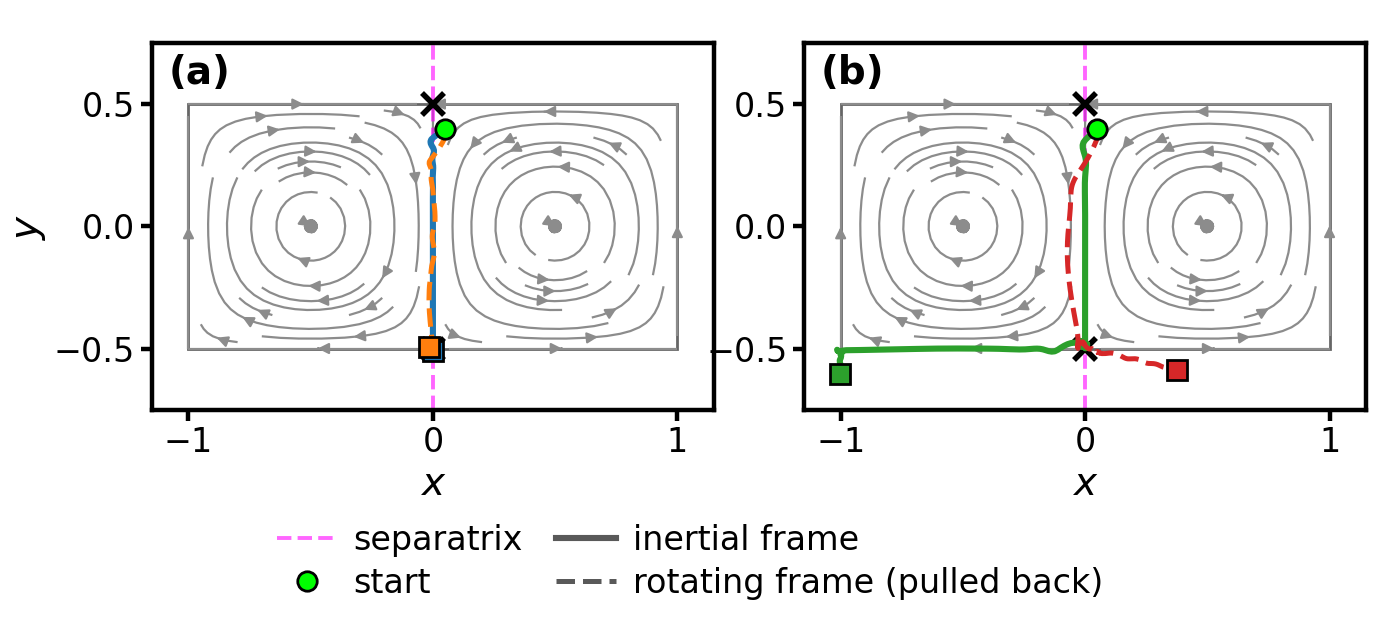
\includegraphics[width=\columnwidth]{figures/objectivity_traverser.png}
    \caption{Objectivity experiment, both controllers started from
    $(0.05, 0.40)$. Each is run in the inertial frame (solid) and in a
    frame rotating at $\Omega = 0.2$ rad/s (dashed, pulled back to
    inertial coordinates). (a) the $s_1$ tracker's two runs coincide
    along the whole separatrix and capture at the same saddle (final gap
    0.025). (b) the $D$ tracker's rotating-frame run leaves the
    separatrix (final gap 1.219), the artifact predicted by
    (\ref{eq:D_not_objective}).}
    \label{fig:oecs_objectivity}
\end{figure}

The rotating-frame experiment of Section~\ref{sec:test_plan} reverses the
ranking, and not by a margin (Fig.~\ref{fig:oecs_objectivity}). The $s_1$
tracker's two runs are the same material path, final gap 0.025 and mean gap
0.014, with mean distance to the true trench network of 0.000 inertial
against 0.005 rotating, both capturing at the same bottom saddle. The $D$
tracker's rotating-frame run does not degrade. It leaves the structure,
reaching a mean trench-network distance ten times its inertial value of
0.005 and a final gap of 1.219 from its inertial twin, ending in the gyre
interior where no structure exists.

This is (\ref{eq:D_not_objective}) in closed loop. The added solid-body
vorticity moves the whole $D'$ landscape, and the same rotation
contaminates the flow measurement that the on-band branch of
(\ref{eq:vpar}) reads, so both terms of (\ref{eq:d_law}) are steered by a
frame artifact rather than by the field. No gain recovers this, because the
artifact is in the surrogate. The $s_1$ tracker inherits the protection of
Proposition~\ref{prop:equivariance} instead, which exempts one instant and
holds only up to the frame-transport term, so a small nonzero gap is what
it predicts rather than a violation of it. The experiment bounds that
residue at 0.025 over a full run without separating its sources.

Objectivity is not free, and the double gyre is the wrong field on which to
price it. Objectivity buys no extra reach there, since the two trenches
coincide for the reason given in Section~\ref{sec:disc_clean}, and the
identically vanishing shear keeps $r$ away from zero, so the $1/r$ exposure
a generic field loads is barely tested. What the double gyre does expose is
rate. The $D$ tracker normalizes by a curvature and holds $a_\perp = 1$
along the whole structure. The $s_1$ tracker has no curvature to normalize
by (Remark~\ref{rem:s1hess}), so it takes $a_\perp = g_\perp\kappa_\perp$
from the field, and at the operating point of Table~\ref{tab:params} that
puts the outer half of the structure past the discrete stability threshold
(Table~\ref{tab:bandwidth}). The five-fold zero-noise tracking-error gap of
Section~\ref{sec:disc_noise} is that cost, measured.

The ladder (\ref{eq:gain_ladder}) places both surrogates on the same rung,
so the choice between them is not one of accuracy. It is which channels
carry constants. Everything derived from $\hat{D}$ carries the observer
term $O(\mathrm{Ro})$, and $\hat{\mathbf{H}}_D$ carries the
unmodelled-derivative floor $e$ as well, while $\hat{s}_1$ carries neither
and is exposed instead at $1/r$, which belongs to the strain field rather
than to the sensing. The rotating-frame gaps contain no $\nu$, no
$\tilde{\rho}$, and no formation geometry, so no estimator improvement
removes them. Objectivity is therefore free at the estimator and paid at
the controller, in the Newton normalization Remark~\ref{rem:s1hess}
forbids. One derivative order runs the other way and partly offsets that
cost. The tangent the $s_1$ tracker rides comes from the
\emph{first-order} fitted coefficients, one order better in noise gain than
the $\hat{\mathbf{H}}_D$ eigenvectors the $D$ tracker uses for the same
purpose, $4.5^\circ$ against $41^\circ$ at $\sigma_{uv} = 0.01$
(Section~\ref{sec:results_est}).

\subsection{Behavior on a Measured Field}
\label{sec:disc_ocean}

\begin{figure}[!t]
    \centering
    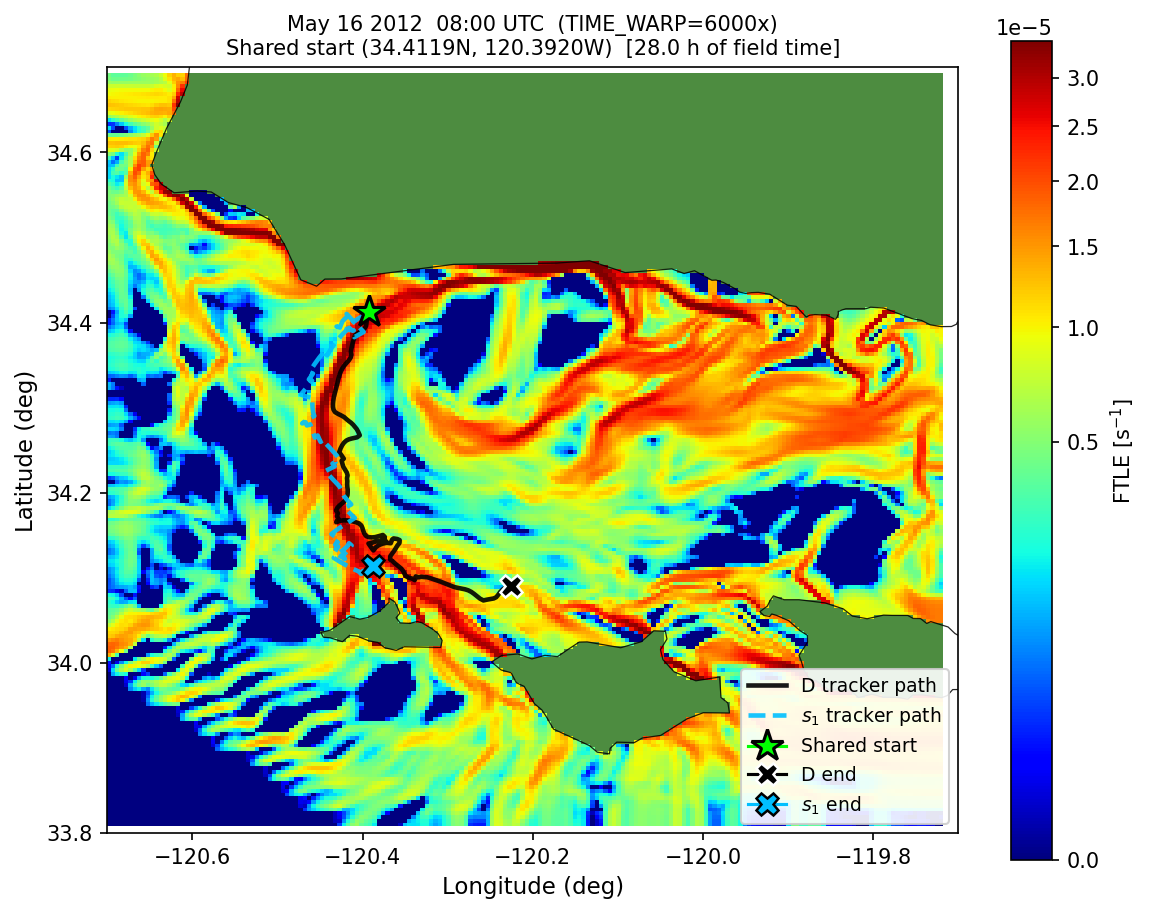
\includegraphics[width=0.38\textwidth]{figures/ocean_ftle_trajectory_overlay_2km.png}
    \caption{28-h $D$ and $s_1$ tracker paths, from a single shared
    start, over the 24-h forward FTLE field computed offline from the
    same 2~km data. Both paths follow the dominant ridge from the
    channel entrance to the bifurcation and separate only near
    landfall, where the $D$ tracker reaches the middle island's north
    coast and the $s_1$ tracker is still converging on the same target
    when the 28-h record ends.}
    \label{fig:ocean_ftle}
\end{figure}

The ocean record removes the coincidence Section~\ref{sec:disc_clean} rests
on. A measured field has no reason to carry a vorticity-free trench
network, so (\ref{eq:trench_coincide}) no longer forces the two surrogates
onto a common curve. Both trackers were run unmodified from a single shared
start north of the channel entrance,
$(34.41^{\circ}\mathrm{N}, -120.39^{\circ}\mathrm{W})$, at the operating
point of Table~\ref{tab:params}. Over the 28~h trial both descend through
the channel entrance and track the same ridge through the bifurcation,
their paths overlapping for nearly the entire record, and they separate
only in the final stretch, where the $D$ tracker continues to landfall on
the middle island's north coast while the $s_1$ tracker is still closing on
the same target when the budget ends.

What survives the loss of pointwise agreement is the corridor.
Fig.~\ref{fig:ocean_ftle} places both trials against the 24-h forward-time
FTLE field, computed offline over the same window in the style of
\cite{25}. Both follow the dominant ridge from the channel entrance to the
bifurcation closely, without that ridge being available to either
controller at any point, since only the local estimates built from the
current samples at the formation enter the commands. Recomputing that field
at four anchor times across the record confirms that the dominant ridge
persists while the finer structure downstream evolves, and the $D$
tracker's outcome is not knife-edge sensitive to the start, with 84 of 100
jittered starts landing on the same middle-island branch. Two controllers
reading different halves of the same splitting identity, from a shared
start on a measured field, agree on which corridor the transport skeleton
occupies while disagreeing about the trajectory inside it.

That agreement is empirical, and its scope should be stated plainly.
Instantaneous criteria of this kind are not in general reliable indicators
of the material transport skeleton \cite{24}. The double gyre is a
favorable special case, and this is a finding on one record rather than a
guarantee that carries to arbitrary flows. The record is also genuinely
time-varying, with each controller seeing only the instantaneous samples at
its own formation position and no analytic guarantee offered for that case.

The field is generic in a second way that matters for the $s_1$ tracker. It
has isolated degeneracies and cores that move between frames, so the
experiment exercises tangent selection (\ref{eq:tangent_select}) where
neither the eigenframe nor the trench network is axis-aligned, which the
double gyre cannot do. It offers no genuine two-dimensional minimum of
$s_1$ within reach of the ride, so the reachability condition of Problem 2
does not engage and (\ref{eq:capture_test}) never fires. That non-firing is
an outcome of the law rather than a failure of it, and it closes the
terminal argument of Section~\ref{sec:disc_clean} from the other side.
Absent a stationary point of $s_1$ close enough to the ride, the same
unmodified controller behaves as a traverser, reading the ridge structure
from the objective strain term alone. Which of the two behaviors appears,
capture on the double gyre and traverse on the ocean, is a property of the
field and not of a setting, since the terminal test is unconditional by
design and has no mode to select.

\subsection{Selection Rule}
\label{sec:selection}

Read together, the four conditions give a selection rule. On a clean
field in an inertial frame the two trackers are interchangeable, and
(\ref{eq:trench_coincide}) says when that holds exactly. With a noisy
sensor in an inertial frame the $D$ tracker holds a grid step longer
and fails by decay rather than by inversion, which also makes its
failures easier to detect from the recorded quantities. Under a
rotating or otherwise non-inertial observer the $D$ tracker does not
degrade but leaves the structure, and only the $s_1$ tracker returns
the same material path. On a generic measured field either recovers the
corridor, so the choice there returns to the first three
considerations. Both consume the same fit, so the switch costs one
function call rather than a new estimator or formation.

\subsection{Limitations}
\label{sec:limitations}

Tracking a trench is structurally harder than tracking a regular level set.
A level set is fixed by first-order information, while a trench lives
exactly where that gradient vanishes in the normal direction, so controller
and proof alike must synthesize the missing direction from curvature. The
eigenstructure dependence, mode switching, and tube assumptions of
Section~\ref{sec:stability} are the price. Three further conditions sit
outside that analysis. The fit is ill-conditioned whenever the six sampling
points drift toward a common conic (Proposition~\ref{prop:conic}), for
which monitoring $\kappa(\boldsymbol{\Phi})$ and adding a
shape-maintenance term is the direct mitigation, not implemented here.
Noise can chatter the $D$ tracker across the band boundary
(\ref{eq:flow_band}), which costs only along-trench speed, since both
branches of (\ref{eq:vpar}) share the transverse dynamics
(\ref{eq:n_dynamics}). Third, the strain eigenframe is fragile where
$\mathbf{S}$ approaches isotropy, the $1/r$ exposure of
Section~\ref{sec:sensitivity}. Tangent selection (\ref{eq:tangent_select})
is the defense once the ride is underway, comparing gradient alignment
rather than eigenvector identity, and the residual risk of a wrong branch
at a crossing under heavy noise is damped but not excluded by the latch on
(\ref{eq:capture_test}).

The $s_1$ tracker's tangent seed is the sharpest of the design limitations,
and Section~\ref{sec:disc_noise} gives its mechanism. Four unimplemented
alternatives trade it differently. A fixed world-axis component of
$\mathbf{e}_2$ removes the flow dependence at the cost of an arbitrary
discontinuity and makes the law memoryless. A team with a trusted heading
resolves the sign against the world axis at every step at no cost in
objectivity, since $s_1$ and its eigenframe are objective whether or not
the sign is anchored externally. A confidence check on the seed converts a
wrong commitment into a longer settling phase, and re-fitting the sign over
several early steps trades the single-instant risk for a short transient of
ordinary tracking-error exposure. None was implemented, since the finding
was made late enough in the noise-sweep validation that a design change
here would need its own noise sweep to verify.

No controlled head-to-head against the straddle family \cite{17,18,19} or
the onboard-FTLE strategy of \cite{21} was run, and two grounds keep the
comparison of Section~\ref{sec:related_robots} structural rather than
empirical. First, initialization is not a detail of those methods but the
premise of their guarantees. \cite{17}'s straddling formation control is
stated for robots already on opposite sides of the boundary, and \cite{21}
assumes the center robot starts on $B_u$, so running either from an
off-structure start is outside its own stated problem. Second, the two
plants differ. \cite{17,18,19,20} and \cite{21} both write the robot's
velocity as the commanded term plus the ambient flow (their eq.~1a in
\cite{17}, eq.~5a in \cite{21}), so their robots are advected, while this
paper's are not (Section~\ref{sec:problem_statement}). One simulator cannot
host both without altering one of them.

All results are from simulation, and hardware validation on the Decabot
testbed is planned as a follow-on study. Throughout, robot motion is
commanded by the control law, not advected by the sampled flow
(Section~\ref{sec:problem_statement}). For the Decabot testbed this is
exact rather than approximate, since the robots are not immersed in
anything and the field is encoded and read rather than physically
experienced \cite{40}. On the ocean field it is an extrapolation. The
commanded speed cap is far above realized ocean currents at this operating
point, but the assumption itself is untested against real advection and is
a scope boundary for that experiment, not a validated one.

\subsection{Future Work}
\label{sec:future}

A time-derivative correction term, analyzed against the analytic
$\varepsilon > 0$ double gyre, would extend the stability results to
time-varying fields with a quantified bound. Online formation reshaping
would protect the conditioning of $\boldsymbol{\Phi}$, and a step-halving
sweep would separate the $s_1$ tracker's discretization limit cycle from
its estimation error (Table~\ref{tab:bandwidth}). Hardware deployment on
the Decabot testbed would test the no-advection assumption directly.
Extension to three dimensions raises the estimation stakes to ten
coefficients per component, so ten robots or a reduced-order estimator.
Targets other than critical points, transient attracting profiles and eddy
cores among them, are a natural next object for the same estimator.



\section{Conclusion}
\label{sec:conclusion}


This paper presented one cooperative estimator and two trackers built
on it. A six-robot formation, proved minimal for the unconstrained
quadratic model (Proposition~\ref{prop:minimality}), recovers the local
quadratic model of a planar flow from a single synchronous sample, and
with it both terms of the splitting identity $D = \omega^2/4 - s_1^2$,
with closed-form, heading-isotropic noise gains verified to $2.1\%$.
The $D$ tracker solves Problem 1, riding the connected trench network of
$D$ on a modified Newton step, with a Lyapunov certificate and a
network-traversal theorem. The $s_1$
tracker solves Problem 2, riding the same network from the strain term
alone, with a terminal test built only from the objective gradient.
That test is available because $s_1$'s minimum is recoverable from a
first derivative of the
fit, where $D$'s needs a curvature the estimator returns with neither a
reliable magnitude nor, past a low noise level, a reliable eigenframe
(Remark~\ref{rem:s1hess}, Section~\ref{sec:sensitivity}). Its frame
equivariance was demonstrated in closed loop rather than asserted, the
same material curve in either observer frame (gap 0.025), where the $D$
tracker follows a frame artifact (gap 1.219). Monte Carlo sweeps placed
the $D$ tracker's failure cliff within 5\% of the estimator's
gradient-reliability threshold, with the curvature eigenframe already
indistinguishable from a random axis there, so the estimator, not the
control law, sets its noise ceiling. The $s_1$ tracker's own noise ceiling is set
one level earlier by a different mechanism, the reliability of the
one-time flow-seeded tangent sign rather than the estimator's gradient
accuracy. On
real Santa Barbara Channel currents the $D$ tracker followed a coherent
ridge for 28 hours to a consistent landfall reproduced by 84 of 100
nearby starts, and the $s_1$ tracker, started on that same ridge, rode
the same network structure for 28 hours from the objective strain term
alone. The choice between the two trackers is set by the observing
platform rather than by the flow. Where a team can certify its
orientation against a trusted external reference, the $D$ tracker
tolerates the noisier sensor. Where it cannot, only the $s_1$ tracker
returns the same material curve. Both read the same fit, so a team that
carries the estimator carries both.

\appendices

\section{Cluster Space Variables for the Six-Robot Formation}
\label{app:cluster_vars}

The cluster controller of Section~\ref{sec:arch} acts on a twelve-element
cluster pose, three variables locating and orienting the formation and
nine describing its shape. Robots are grouped into three pairs,
$\{1,2\}$, $\{3,4\}$, and $\{5,6\}$, whose midpoints $\mathbf{m}_A$,
$\mathbf{m}_B$, $\mathbf{m}_C$ (components $m_{\bullet x}$,
$m_{\bullet y}$) form a triangle in the side-angle-side form standard
in cluster space work \cite{37,38}. With $\mathbf{p}_i = (x_i, y_i)$
the position of robot $i$, the forward position kinematics are
\begin{align}
    x_c &= \frac{1}{6}\sum_{i=1}^{6} x_i,
    \label{eq:ck_xc}\\
    y_c &= \frac{1}{6}\sum_{i=1}^{6} y_i,
    \label{eq:ck_yc}\\
    \theta_c &= \operatorname{atan2}
    \left(m_{Ay} - m_{By},\; m_{Ax} - m_{Bx}\right),
    \label{eq:ck_thetac}\\
    p_1 &= \lVert \mathbf{m}_B - \mathbf{m}_A \rVert,
    \label{eq:ck_p}\\
    q_1 &= \lVert \mathbf{m}_C - \mathbf{m}_B \rVert,
    \label{eq:ck_q}\\
    \beta_1 &= \arccos\!\left(
    \frac{p_1^2 + q_1^2 - r_1^2}{2\,p_1 q_1}\right),
    \quad r_1 = \lVert \mathbf{m}_A - \mathbf{m}_C \rVert,
    \label{eq:ck_beta}\\
    L_2 &= \lVert \mathbf{p}_2 - \mathbf{p}_1 \rVert,
    \label{eq:ck_L2}\\
    \theta_2 &= \operatorname{atan2}(y_2 - y_1,\; x_2 - x_1),
    \label{eq:ck_th2}\\
    L_3 &= \lVert \mathbf{p}_4 - \mathbf{p}_3 \rVert,
    \label{eq:ck_L3}\\
    \theta_3 &= \operatorname{atan2}(y_4 - y_3,\; x_4 - x_3),
    \label{eq:ck_th3}\\
    L_4 &= \lVert \mathbf{p}_6 - \mathbf{p}_5 \rVert,
    \label{eq:ck_L4}\\
    \theta_4 &= \operatorname{atan2}(y_6 - y_5,\; x_6 - x_5).
    \label{eq:ck_th4}
\end{align}
These symbols are local to the cluster controller layer, and some are
spelled like symbols used elsewhere for unrelated quantities: $p$ and
$q$ as expansion orders in (\ref{eq:error_budget}), $\beta$ as the ride
flag in (\ref{eq:oecs_law}), and the Jacobian below, which is not the
flow velocity gradient $\mathbf{J}$ of (\ref{eq:jacobian}). The layered
architecture of Section~\ref{sec:arch} keeps them apart, since each layer
holds its own state and only $\mathbf{p}_c$ and $\dot{\mathbf{p}}_c$
cross the boundary, but the reuse still warrants care.

The inverse kinematics can be found geometrically, and the Jacobian and
inverse Jacobian follow in the normal way \cite{37}, giving the
$12 \times 12$ matrices that map robot velocities into cluster
velocities for feedback and cluster velocities into robot velocities
for command.

\begin{thebibliography}{99}
\bibitem{1} J. Cortés and M. Egerstedt, ``Coordinated control of multi-robot
systems: A survey,'' \textit{SICE Journal of Control, Measurement, and
System Integration}, vol. 10, no. 6, pp. 495--503, 2017.

\bibitem{2} P. Ögren, E. Fiorelli, and N. E. Leonard, ``Cooperative control
of mobile sensor networks: Adaptive gradient climbing in a distributed
environment,'' \textit{IEEE Transactions on Automatic Control}, vol. 49, no. 8,
pp. 1292--1302, 2004.

\bibitem{3} R. T. McDonald, C. A. Kitts, and M. A. Neumann, ``Navigation of
scalar fronts with multirobot clusters in simulation and experiment,''
\textit{IEEE Systems Journal}, vol. 14, no. 3, pp. 3755--3766, 2020.

\bibitem{4} C. A. Kitts, R. T. McDonald, and M. A. Neumann, ``Adaptive
navigation control primitives for multirobot clusters: Extrema finding,
contour following, ridge/trench following, and saddle point station keeping,''
\textit{IEEE Access}, vol. 6, pp. 17625--17642, 2018.

\bibitem{5} R. T. McDonald, C. A. Kitts, and M. A. Neumann, ``Experimental
implementation and verification of scalar field ridge, trench, and saddle
point maneuvers using multirobot adaptive navigation,'' \textit{IEEE Access},
vol. 7, pp. 62950--62961, 2019.

\bibitem{6} L. Briñón-Arranz, A. Renzaglia, and L. Schenato, ``Multirobot
symmetric formations for gradient and Hessian estimation with application to
source seeking,'' \textit{IEEE Transactions on Robotics}, vol. 35, no. 3,
pp. 782--789, 2019.

\bibitem{7} M. Mateus, R. Canelas, L. Pinto, and N. Vaz, ``When
tragedy strikes: Potential contributions from ocean observation to
search and rescue operations after drowning accidents,'' \textit{Front.
Mar. Sci.}, vol. 7, art. 55, 2020.

\bibitem{8} P. Keramea, K. Spanoudaki, G. Zodiatis, G. Gikas, and
G. Sylaios, ``Oil spill modeling: A critical review on current trends,
downscaling, and applications,'' \textit{J. Mar. Sci. Eng.}, vol. 9,
no. 2, art. 181, 2021.

\bibitem{9} C. Waight and C. A. Kitts, ``Adaptive navigation of multirobot
systems to critical points in 2D vector fields,'' submitted for publication.

\bibitem{10} J. Das, F. Py, T. Maughan, T. O'Reilly, M. Messié, J. Ryan,
G. S. Sukhatme, and K. Rajan, ``Coordinated sampling of dynamic oceanographic
features with underwater vehicles and drifters,'' \textit{The International
Journal of Robotics Research}, vol. 31, no. 5, pp. 626--646, 2012.

\bibitem{11} S. McCammon, G. Marcon dos Santos, M. Frantz, T. P. Welch,
G. Best, R. K. Shearman, J. D. Nash, J. A. Barth, J. A. Adams, and
G. A. Hollinger, ``Ocean front detection and tracking using a
team of heterogeneous marine vehicles,'' \textit{Journal of Field Robotics},
vol. 38, no. 6, pp. 854--881, 2021.

\bibitem{12} S. R. Ramp et al., ``Preparing to predict: the second autonomous
ocean sampling network (AOSN-II) experiment in the Monterey Bay,''
\textit{Deep Sea Research Part II: Topical Studies in Oceanography}, vol. 56,
no. 3-5, pp. 68--86, 2009.

\bibitem{13} G. Haller and G. Yuan, ``Lagrangian coherent structures and mixing
in two-dimensional turbulence,'' \textit{Physica D: Nonlinear Phenomena},
vol. 147, no. 3-4, pp. 352--370, 2000.

\bibitem{14} T. Peacock and G. Haller, ``Lagrangian coherent structures: The
hidden skeleton of fluid flows,'' \textit{Physics Today}, vol. 66, no. 2,
pp. 41--47, 2013.

\bibitem{15} S. C. Shadden, F. Lekien, and J. E. Marsden, ``Definition and
properties of Lagrangian coherent structures from finite-time Lyapunov
exponents in two-dimensional aperiodic flows,'' \textit{Physica D}, vol. 212,
no. 3-4, pp. 271--304, 2005.

\bibitem{16} C. Dong et al., ``Oceanic mesoscale eddies,'' \textit{Ocean-Land-
Atmosphere Research}, vol. 4, p. 0081, 2025.

\bibitem{17} M. Michini, M. A. Hsieh, E. Forgoston, and I. B. Schwartz,
``Robotic tracking of coherent structures in flows,'' \textit{IEEE Transactions
on Robotics}, vol. 30, no. 3, pp. 593--603, 2014.

\bibitem{18} M. Michini, H. Rastgoftar, M. A. Hsieh, and S. Jayasuriya,
``Distributed formation control for collaborative tracking of manifolds in
flows,'' in \textit{Proc. American Control Conference}, pp. 3874--3880, 2014.

\bibitem{19} M. Michini, M. A. Hsieh, E. Forgoston, and I. B. Schwartz,
``Experimental validation of robotic manifold tracking in gyre-like flows,''
in \textit{Proc. IEEE/RSJ International Conference on Intelligent Robots
and Systems (IROS)}, pp. 2306--2311, 2014.

\bibitem{20} G. Knizhnik, P. Li, X. Yu, and M. A. Hsieh, ``Flow-based control
of marine robots in gyre-like environments,'' in \textit{Proc. 2022 Int. Conf.
on Robotics and Automation (ICRA)}, pp. 3047--3053, 2022.

\bibitem{21} D. Kularatne and M. A. Hsieh, ``Tracking attracting manifolds in
flows,'' \textit{Autonomous Robots}, vol. 41, no. 8, pp. 1575--1588, 2017.

\bibitem{22} R. N. Smith, M. Schwager, S. L. Smith, B. H. Jones, D. Rus,
and G. S. Sukhatme, ``Persistent ocean monitoring with underwater gliders:
Adapting sampling resolution,'' \textit{J. Field Robotics}, vol. 28, no. 5,
pp. 714--741, 2011.

\bibitem{23} J. Das, F. Py, T. Maughan, T. O'Reilly, M. Messi\'e, J. Ryan,
G. S. Sukhatme, and K. Rajan, ``Coordinated sampling of dynamic
oceanographic features with underwater vehicles and drifters,''
\textit{Int. J. Robot. Res.}, vol. 31, no. 5, pp. 626--646, 2012.

\bibitem{24} G. Haller, ``Lagrangian coherent structures,'' \textit{Annual
Review of Fluid Mechanics}, vol. 47, pp. 137--162, 2015.

\bibitem{25} M. Serra and G. Haller, ``Objective Eulerian coherent
structures,'' \textit{Chaos: An Interdisciplinary Journal of Nonlinear
Science}, vol. 26, no. 5, p. 053110, 2016.

\bibitem{26} P. J. Nolan, M. Serra, and S. D. Ross, ``Finite-time Lyapunov
exponents in the instantaneous limit and material transport,''
\textit{Nonlinear Dynamics}, vol. 100, no. 4, pp. 3825--3852, 2020.

\bibitem{27} T. D. Harms, S. T. M. Dawson, and B. J. McKeon, ``Lagrangian
gradient regression for the detection of coherent structures from sparse
trajectory data,'' \textit{Royal Society Open Science}, vol. 11, no. 9,
p. 240586, 2024.

\bibitem{28} G. Haller, ``Dynamic rotation and stretch tensors from a
dynamic polar decomposition,'' \textit{Journal of the Mechanics and Physics
of Solids}, vol. 86, pp. 70--93, 2016.

\bibitem{29} A. Okubo, ``Horizontal dispersion of floatable particles in the
vicinity of velocity singularities such as convergences,'' \textit{Deep-Sea
Research}, vol. 17, no. 3, pp. 445--454, 1970.

\bibitem{30} J. Weiss, ``The dynamics of enstrophy transfer in two-dimensional
hydrodynamics,'' \textit{Physica D: Nonlinear Phenomena}, vol. 48, no. 2-3,
pp. 273--294, 1991.

\bibitem{31} J. C. R. Hunt, A. A. Wray, and P. Moin, ``Eddies, streams, and
convergence zones in turbulent flows,'' in \textit{Proc. Summer Program,
Center for Turbulence Research}, Rep. CTR-S88, pp. 193--208, 1988.

\bibitem{32} B.-L. Hua and P. Klein, ``An exact criterion for the stirring
properties of nearly two-dimensional turbulence,'' \textit{Physica D}, vol. 113,
no. 1, pp. 98--110, 1998.

\bibitem{33} R. Cooper, D. Rajabhandharaks, R. T. McDonald, M. A. Neumann,
and C. A. Kitts, ``Initial study of multirobot adaptive
navigation for exploring environmental vector fields,'' in \textit{Proc.
IEEE Aerospace Conference}, 2019.

\bibitem{34} Y. N. Dauphin, R. Pascanu, C. Gulcehre, K. Cho, S. Ganguli,
and Y. Bengio, ``Identifying and attacking the saddle point problem in
high-dimensional non-convex optimization,'' in \textit{Advances in Neural
Information Processing Systems}, vol. 27, pp. 2933--2941, 2014.

\bibitem{35} W. Yao, H. G. de Marina, B. Lin, and M. Cao,
``Singularity-free guiding vector field for robot navigation,''
\textit{IEEE Trans. Robot.}, vol. 37, no. 4, pp. 1206--1221, 2021.

\bibitem{36} T. Liddy and T.-F. Lu, ``Obstacle avoidance using complex
vector fields,'' in \textit{Proc. Australasian Conf. Robotics and
Automation (ACRA)}, 2008.

\bibitem{37} C. A. Kitts and I. Mas, ``Cluster space specification and control
of mobile multirobot systems,'' \textit{IEEE/ASME Transactions on Mechatronics},
vol. 14, no. 2, pp. 207--218, 2009.

\bibitem{38} T. Adamek, C. A. Kitts, and I. Mas, ``Gradient-based cluster space
navigation for autonomous surface vessels,'' \textit{IEEE/ASME Transactions on
Mechatronics}, vol. 20, no. 2, pp. 506--518, 2014.

\bibitem{39} S. Tomer et al., ``A low-cost indoor testbed for multirobot
adaptive navigation research,'' in \textit{Proc. IEEE Aerospace Conference},
pp. 1--12, 2018.

\bibitem{40} C. Waight and C. Kitts, ``A functional indoor testbed for
multirobot adaptive navigation in vector field environments,'' in
\textit{Proc. ASME Int. Design Engineering Technical Conf. and Computers
and Information in Engineering Conf.}, vol. 89251, 2025.

\bibitem{41} NOAA National Centers for Environmental Information,
``Near-real-time surface ocean velocities derived from HF-radar stations
located along coastal waters of North Slope Alaska, Gulf of Alaska,
Puerto Rico/Virgin Islands, eastern U.S./Gulf of America, Hawaii, Great
Lakes, and western U.S.,'' NCEI Accession
gov.noaa.nodc:IOOS-HFRadarRTVector.

\bibitem{42} M. Serra, P. Sathe, I. Rypina, A. Kirincich, S. D. Ross,
P. Lermusiaux, A. Allen, T. Peacock, and G. Haller, ``Search and rescue
at sea aided by hidden flow structures,'' \textit{Nature Communications},
vol. 11, no. 1, p. 2525, 2020.

\end{thebibliography}

\end{document}
